\chapter{High-SNR Radar Signal} % Write in your own chapter title
\label{ch:cft} % Add a label in case you want to refer to the chapter.
\section{Introduction}
Radio detection and ranging (radar) system is originally designed for military detection of large aircraft by emitting electromagnetic waves and evaluating the reflections. The follow-up research has investigated the civilian use of radar systems for contactless sensing in various scenarios, such as autonomous driving~\cite{yao2023waterscenes} and human monitoring~\cite{zhang2023overview}. Over the past decade, radar-based sensing has been empowered by deep neural networks to process non-stationary reflected signals or high-dimensional data, enabling versatile applications to replace contact- or visual-based measurement for convenience or privacy concerns (e.g., vital sign monitoring~\cite{liu2024diversity}, gesture recognition~\cite{song2025dual}, fault diagnosis~\cite{chen2024two}).

Radar-based vital sign monitoring, as a popular branch of radar-based sensing, has been explored for decades to measure heart rate or respiration rate in a contactless manner~\cite{zhang2023overview}, and some further studies leverage the deep neural network to realize domain transformation from cardiac mechanical activities (i.e., heartbeat) to electrical activities (i.e., electrocardiogram (ECG)), providing a fine-grained cardiac measurement for wellness monitoring or clinical diagnosis~\cite{zhao2024mmarrhythmia,zhang2024radarODE,zhang2024radarODE-MTL,chen2022contactless,zhang2025horcrux,li2024radarnet,wu2023contactless}. In the literature, radar-based ECG recovery is only realized by deep-learning-based methods, because the domain transformation is extremely complex to be modeled mathematically while such transformation can be learning by deep learning model due to the great nonlinear mapping ability~\cite{chen2022contactless}.

Similar to other research fields involved with deep learning, radar-based ECG recovery also asks for numerous radar signals to train the deep learning model with synchronous ECG ground truths~\cite{li2024radarnet,zhang2024radarODE-MTL,chu2024vessel}. According to previous research, the performance of the deep learning model degrades heavily after reducing $30\%$ of the training data even after applying proper data augmentation techniques~\cite{zhang2025horcrux}, causing difficulties for the deployment in new scenarios due to the demand for hours of ECG collection~\cite{zhang2024radarODE}. However, the method for reducing dependence on data quantity is rarely investigated for radar-based ECG recovery, and all the deep-learning-based ECG recovery models are trained in a supervised manner with large dataset containing $3-32$ hours of synchronous radar-ECG pairs~\cite{chen2022contactless,zhao2024airecg,li2024radarnet}.  

In contrast, most studies are dedicated to inventing advanced signal processing algorithms to enhance the signal quality, because the deep learning model for ECG recovery is vulnerable to the inputs contaminated by noises and requires high signal-to-noise ratio (SNR) radar signals as inputs~\cite{chen2022contactless,liu2024diversity}. The methods for capturing high-SNR radar signals can be categorized into two groups:
\begin{itemize}
\item The first type of method focuses on designing advanced radar front-end with multiple transmitters (Tx) and receivers (Rx)~\cite{li2024robust,xiong2022vital} or calibrating baseband radar signals from in-phase and quadrature (IQ) channels to a circular shape~\cite{dong2024robust,ni2024accurate,zhang2024single}.
\item The second type of method assumes that the rough localization of human body provides accurate chest region with the majority of range bins containing useful cardiac features, and high-SNR signal can be obtained by selecting useful bins/channels/antennas~\cite{li2024radarnet,zhang2025umimo}, applying clustering algorithms~\cite{chen2022contactless} or accumulating the signals from various dimensions (e.g., chirps, frames, antennas)~\cite{liu2024diversity}. 
\end{itemize}

The first type of method is not suitable for some commonly used frequency-modulated continuous-wave (FMCW) radar platforms (e.g., TI AWR-x radar) due to the on-board digital front-end module filtering the frequency-modulated feature of baseband signal (i.e., circular IQ plot)~\cite{chen2024co}, preventing the broad applications of this approach in commercial radar. The second type of method relies on accurate localization of the chest region, while the existing methods only provide a rough location of the human body, causing a deviation of several decimeters due to different postures of the subject~\cite{chen2021movi}. Therefore, the methods based on signal accumulation may fail because only a minority of range bins contain cardiac features, hence not subjecting to the law of large numbers~\cite{liu2024diversity}. Although some aforementioned studies have proposed methods for selecting or clustering the useful range bins with cardiac features~\cite{chen2022contactless,li2024radarnet}, the computational cost for traversing a large objective space can be huge without an accurate cardiac location.

Based on the above discussion, it is still a challenge to: (a) precisely locate and track the cardiac location during data collection to efficiently extract high-SNR radar signal; (b) develop a deep learning framework for radar-based ECG recovery, with less demand for ECG collection and realizing an efficient model training especially for new scenarios with limited data. To overcome these two challenges, the contributions of this study can be listed as: 
\begin{itemize}
\item A cardio-focusing and -tracking (CFT) algorithm is proposed based on derivative-free optimization (DFO) to find the cardio-focused (CF) point by iteratively evaluating the potential points in a discontinuous objective space, with a universal signal template designed to adaptively assess the signal SNR as costs.
\item A transfer learning framework RFcardi is proposed following a self-supervised learning (SSL) paradigm to effectively learn the latent representations from radar signals by leveraging an appropriate pre-text task. Accordingly, this work further designates the sparse signal recovery (SSR) as the pre-text task, assisting the RFcardi to learn essential representations for the later ECG recovery.
\item The proposed CFT algorithm has been validated on sitting subjects in various scenarios and could provide radar measurements with better SNR compared with existing methods. In addition, the pre-trained RFcardi framework can be easily adapted to realize radar-based ECG recovery with a small amount of synchronous radar-ECG measurements for fine-tuning. 
\end{itemize}

The rest of the paper is organized as follows. Section~\ref{sec:rw} provides the background information for radar-based ECG recovery and SSL. Section~\ref{sec:method} elaborates the proposed CFT algorithm and RFcardi framework, with the experimental settings and results shown in Section~\ref{sec:exp} and~\ref{sec:result}. The final conclusion is shown in Section~\ref{sec:conclusions}.

\section{Theoretical Background and Challenges}\label{sec:rw}
\subsection{FMCW Radar Foundations}
FMCW radar has been widely used in nowadays millimeter-wave (mmWave) sensing to measure the range, velocity and angle of arrival (AoA) of the objects appearing in the field of view~\cite{tang2024bsense}, with three critical concepts that configure the transmitted waveform:
\begin{itemize}
\item \textbf{Chirp } is the minimum component in the FMCW signal with microsecond-level duration and is often called fast time. The waveform of a single chirp is a sinusoidal signal with frequency that changes linearly over time, with the key characteristics designated by start frequency, bandwidth and chirp duration to get range information of the object.
\item \textbf{Frame} is a collection of multiple chirps that forms a complete observation window to get the velocity information based on the range bins extracted from chirps and is often referred to as slow time.
\item \textbf{Virtual antenna array (channel)} is a commonly used concept in multiple-input and multiple-out (MIMO) radar systems and is able to realize complex modulations or beamforming~\cite{xiong2022vital}. However, this study mainly leverages the phase difference across antenna channels to estimate the AoA of the objects.
\end{itemize}
The popular commercial radar platforms have provided a convenient interface for radar configuration,  signal modulation and demodulation~\cite{AWR1843}. Therefore, detailed equations of FMCW radar signal processing might be redundant in this paper, while the theoretical explanation can be found in previous papers~\cite{wang2021mmhrv,tang2024bsense}.

\subsection{Cardiac Signal Extraction from FMCW Radar}
ECG recovery relies on the high-SNR radar inputs that describe the mechanical cardiac activities, and the reflected signal from a given point $E=(x,y,z)$ in 3D space can be expressed as:
\begin{equation}\label{equ:raw_sig}
R(E, t)=\sum_{v=1}^V \sum_{c=1}^C \sum_{n=1}^N s_{v, c, n}(t)\cdot e^{j 2 \pi \frac{2k\cdot d(E, v)}{\text{light speed}} n} \underbrace{e^{j 2 \pi \frac{2\cdot d(E, v)}{\lambda}}}_{\text{phase term}\ \phi}
\end{equation}
where $(x,y,z)$ represents the (horizontal, radial, vertical) axis, $V$ is the number of virtual antenna channels, $C$ means the number of chirps within one frame, $N$ is the total sample points within one chirp, $s_{v, c, n}(t)$ denotes the original received signal, $k$ is the slope of frequency raising, $\lambda$ means wavelength and $d(E, v)$ represents the distance between point $E$ and virtual antenna $v$~\cite{chen2022contactless}. In FMCW processing for vital sign monitoring, the time sample $t$ corresponds to one frame instead of the sample point $n$, and the signal from different chirps $c$ and antenna channels $v$ will be accumulated to improve SNR~\cite{liu2024diversity}.

The interested term in (\ref{equ:raw_sig}) is the variation of distance $d(E,v)$, because it represents the displacements caused by respiration and heartbeat (without considering any other noise). Therefore, the chest region displacement $h(E, t)$ can be unwrapped from phase variation $\Delta \phi$ as
\begin{equation}\label{equ:phase}
h(E, t) = \frac{\lambda \Delta \phi}{4\pi}
\end{equation}

At last, some common noises, such as respiration and thermal noise, can be easily removed using a band-pass filter and differentiator to make sure that the final $h(E, t)$ mostly contains cardiac-related features from point $E$ as shown in Figure~\subref*{fig:radar_good}. 

\textbf{Challenge: } It is natural to think the high-SNR radar signal can be searched in a constrained space by optimization, while there is no appropriate method to assess the signal SNR in terms of cardiac features contained, and the objective space is actually highly discontinuous with adjacent points may revealing totally different SNR as shown in Figure~\subref*{fig:radar_good} and~\subref*{fig:radar_bad}, restricting the application of common gradient-based optimization algorithms. 

\begin{figure}[tb]
        \centering
        \subfloat[]{\label{fig:radar_good}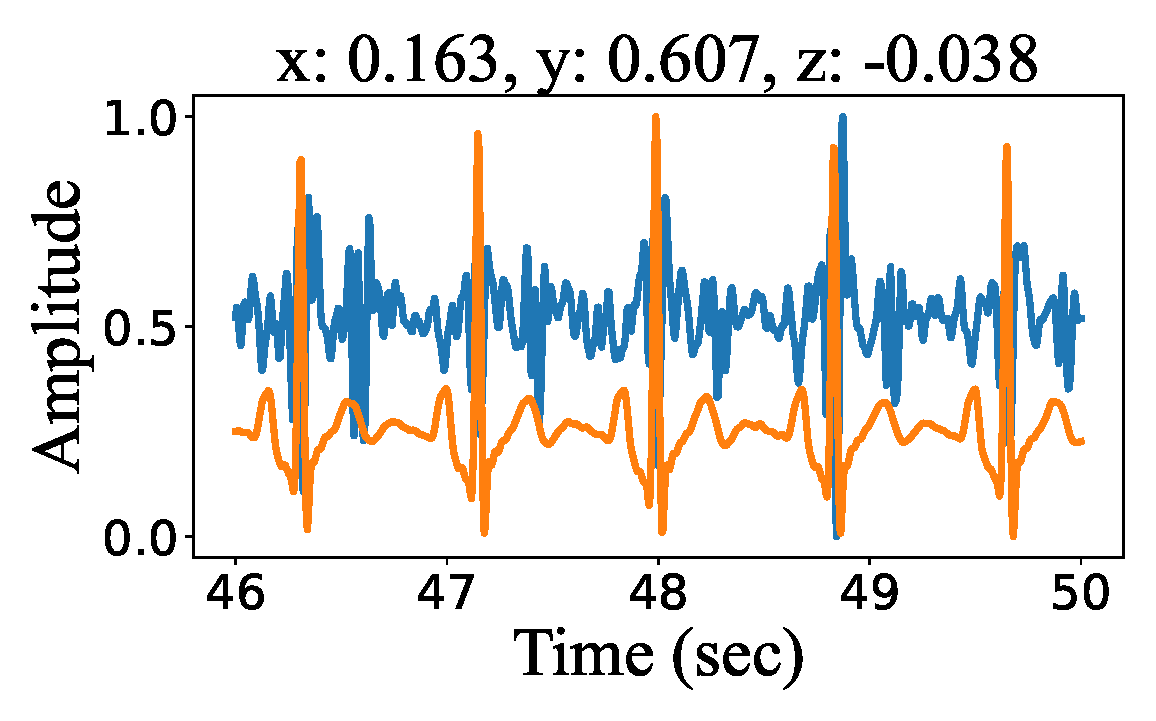
\includegraphics[width=0.25\columnwidth]{radar_good.eps}}
        \subfloat[]{\label{fig:radar_bad}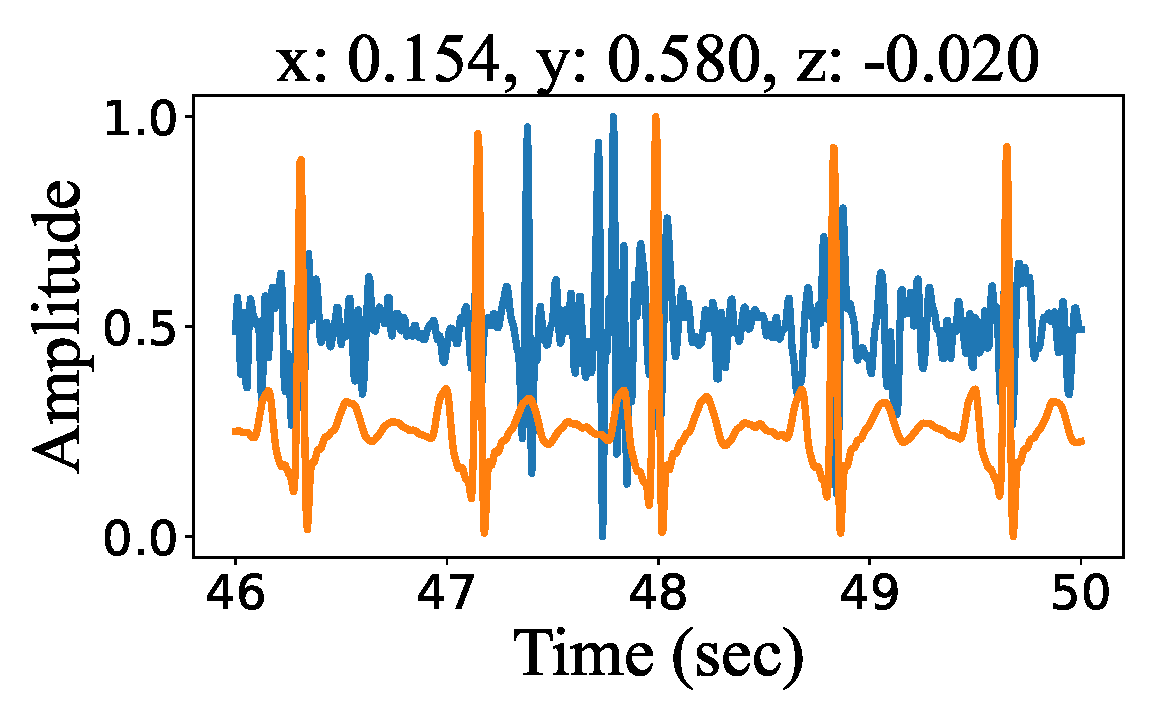
\includegraphics[width=0.25\columnwidth]{radar_bad.eps}}
        \subfloat[]{\label{fig:org_scen}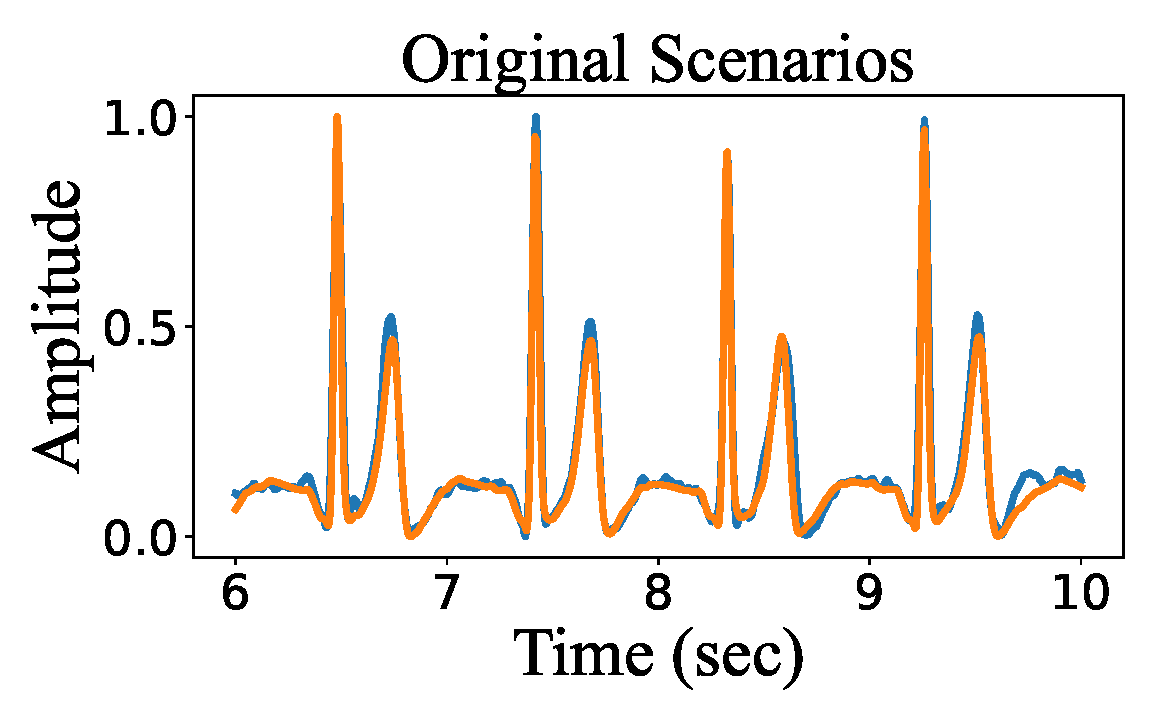
\includegraphics[width=0.25\columnwidth]{org_scen.eps}}
        \subfloat[]{\label{fig:cardi_good}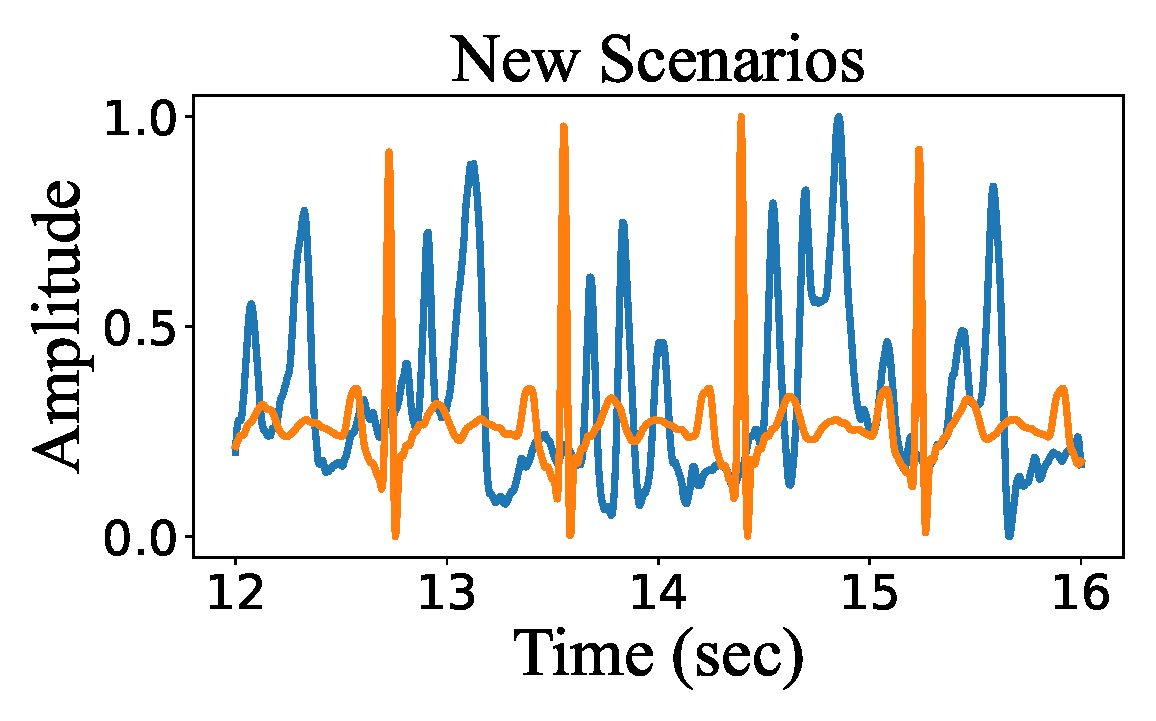
\includegraphics[width=0.25\columnwidth]{cardi_good.eps}}
        \caption{Challenges for radar-based ECG recovery: (a) and (b) Radar signals with high and low SNR for adjacent points with a distance of $0.03$m; (c) and (d) Inference results of a well-trained deep learning model in original and new scenarios.}
        \label{fig:challenges}
\end{figure}

\subsection{Transfer Learning}
In addition to high-SNR radar inputs, accurate ECG recovery also relies on the scale of datasets to train the deep learning model, with the previous research normally adopting the dataset with the length of $3-32$ hours~\cite{chen2022contactless,zhao2024airecg,li2024radarnet}. Unfortunately, the initial experimental results show that the well-trained deep learning model cannot be directly used for the signal collected from new scenarios even using a similar radar configuration as shown in Figure~\subref*{fig:org_scen} and ~\subref*{fig:cardi_good}, because different in-door scenarios and radar configurations may have unknown interference on radar signals~\cite{zhang2023overview}.

Inspired by other signal-based research~\cite{zhang2025umimo,chen2024tfpred}, transfer learning is a promising paradigm to learn the latent representation from unlabeled radar signal to capture basic cardiac features in an SSL manner, reducing the requirement of cumbersome ECG collection. Then, only a small amount of synchronous radar-ECG pairs is required to fine-tune the pre-trained model to realize the ECG recovery for new scenarios.

\textbf{Challenge: } The efficient SSL requires an appropriate design of the pre-text task to help the deep learning model capture essential features that assist ECG recovery, while no existing work has investigated only learning from radar signals without the aid of ECG ground truth. 

\section{Methodology}\label{sec:method}
\subsection{Overview of CFT-RFcardi Framework}
The pipeline of the proposed CFT-RFcardi framework is shown in Figure~\ref{fig:CFTRFcardi} with three steps:
\begin{itemize}
\item The received radar signal will be converted into a standard format in terms of chirp, frame and virtual antenna channel to obtain the general location of the subject, as shown in Figure~\ref{fig:CFTRFcardi}(a).
\item The rough location acts as the initial state for the CFT algorithm, and the points within a constrained space will be evaluated to find the red CF point with best SNR as shown in Figure~\ref{fig:CFTRFcardi}(b).
\item Signals extracted from the ten best points will be converted into spectrograms to pre-train the backbone with SSR as the pre-text task. Then, the same backbone will used for the fine-tuning stage so that the latent representations learned in the pre-trained model can be seemly transferred for the ECG recovery task, as shown in Figure~\ref{fig:CFTRFcardi}(c).
\end{itemize}

In addition, TI-AWR 1843 radar operated at $77$~Ghz with $2$~Tx and $4$~Rx will be used for data collection, enabling $8$ virtual antenna channels for high-quality signal extraction. The detailed scenario descriptions and radar configurations will be provided in Section~\ref{sec:data_coll}.

\begin{figure}[tb] 
    \centering 
    \includegraphics[width=0.9\columnwidth]{CF_Cardi_struct.pdf}
    \caption{Overview of the CFT-RFcardi framework: (a) Rough localization of human body; (b) Use CFT to find CF point and extract high-SNR radar signals; (c) Transfer learning with pre-text task training and fine-tuning stages.}
    \label{fig:CFTRFcardi} 
\end{figure}

\subsection{Rough Localization}
The received radar signal is first formatted as a standard data matrix in terms of different chirps, frames and virtual channels to provide measurement of range, velocity and AoA, respectively. For the current research level of radar-based vital sign monitoring, the subjects are all quasi-static without velocity, and only the range-angle (RA) map will be calculated using fast Fourier transform (FFT) as shown in Figure~\ref{fig:CFTRFcardi}(a), with a detailed illustration of signal waveform and processing shown in Figure~\ref{fig:rouch_loc}.

\subsubsection{Range FFT}
According to (\ref{equ:raw_sig}), the signal propagation after transmitting introduces a constant phase shift $\phi_s$ in the received signal and is expressed as 
\begin{equation}\label{equ:range}
\phi_s = \frac{4\pi d_0}{\lambda}
\end{equation}
with $d_0$ representing the distance between radar and human body. Therefore, the distance $d_0$ can be extracted from each received signal along fast time using FFT as shown in Figure~\ref{fig:rouch_loc}(a), and the updated data matrix now reveals the range information, i.e., a static object denoted as blue along slow time axis.

\subsubsection{Angle FFT}
The ability of AoA detection relies on the MIMO system using time division multiplexing (TDM-MIMO), with multiple Tx alternately transmitting chirp signals and the corresponding reflections can be distinguished during receiving as shown in Figure~\ref{fig:rouch_loc}(b). Due to the physical distance varies for different Tx/Rx combinations (i.e., Tx$2$Rx$4$ creates $8$ virtual channels), an extra propagation $\Delta \phi_v$ delay will be introduced as:
\begin{equation}\label{equ:angle}
\begin{aligned}
\Delta \phi_v &= \frac{4\pi d_v}{\lambda} \\
d_v &= l\ sin(\theta)
\end{aligned}
\end{equation}
where $d_v$ represents the extra propagation distance, $l$ means the distance between adjacent antenna channels and $\theta$ is the incident angle. Similar to range FFT, the phase differences across different channels can be used to extract AoA information for each range bin by performing FFT along the channel axis, as shown in red squares in Figure~\ref{fig:rouch_loc}(b).

After combining the FFT results for all chirps and channels, the final RA map for the current time sample (frame) can be obtained as shown in Figure~\ref{fig:rouch_loc}. The same procedure can be repeated along the slow time axis to get the rough human body location for all the time samples, but this study only requires the location obtained from the very first frame as the initial point $E_0$ for CFT algorithm.

\begin{figure}[tb] 
    \centering 
    \includegraphics[width=0.5\columnwidth]{rough_loc.pdf}
    \caption{Procedures for obtaining RA map: (a) Range FFT for chirps along fast time; (b) Angle FFT along virtual channels.}
    \label{fig:rouch_loc} 
\end{figure}

\subsection{Cardio-focusing and -tracking (CFT) Algorithm}
The radar signal for any point can be extracted following (\ref{equ:raw_sig}) and (\ref{equ:phase}), and the search progress from $E_0$ to the best point $E_{b}$ (i.e., CF point with high SNR) requires: (a) an appropriate metric to assess whether the radar signal contains wanted cardiac features; (b) an optimization method that is applicable to the discontinuous objective space based on the assessed SNR values as costs. 

\subsubsection{Template Design for Assessing SNR}
An explicit SNR can be calculated with the known “clean” signal, while the "clean" signal for vital signs normally reveals two prominent vibrations corresponding to the ventricular contraction and relaxation~\cite{zhang2024radarODE}, as shown in Figure~\subref*{fig:target_org}. However, considering the vibrations may have subtle differences due to different scenarios or radar configurations (e.g., noise figure and sampling frequency), a universal template $h_m$ is designed in this study to fit the envelope of the radar signal as: 
\begin{equation}
h_m (t) = a_1 \exp(-\frac{(t-b_1)^2}{2c_1^2}) + a_2 \exp(-\frac{(t-b_2)^2}{2c_2^2})
\end{equation}
with $a_1$, $a_2$ controlling the amplitudes of the peaks, $b_1$, $b_2$ determining the centers of the peaks and $c_1$, $c_2$ adjusting the width of the peaks. In practice, $a_1$ and $b_1$ will be fixed based on the dominant peaks detected as the red points in Figure~\subref*{fig:target_sig}, and other parameters are left to be determined as a simple curve fitting problem. Finally, the mean square error (MSE) between the radar signal envelope and the synthetic template is reckoned to be an assessment of signal SNR as shown in Figure~\subref*{fig:target_sig}, because fewer components could fit the designed template for low-SNR radar signal without obvious cardiac features, as shown in Figure~\subref*{fig:target_org_bad} and~\subref*{fig:target_sig_bad}.

\begin{figure}[tb]
  \centering
  \subfloat[]{\label{fig:target_org}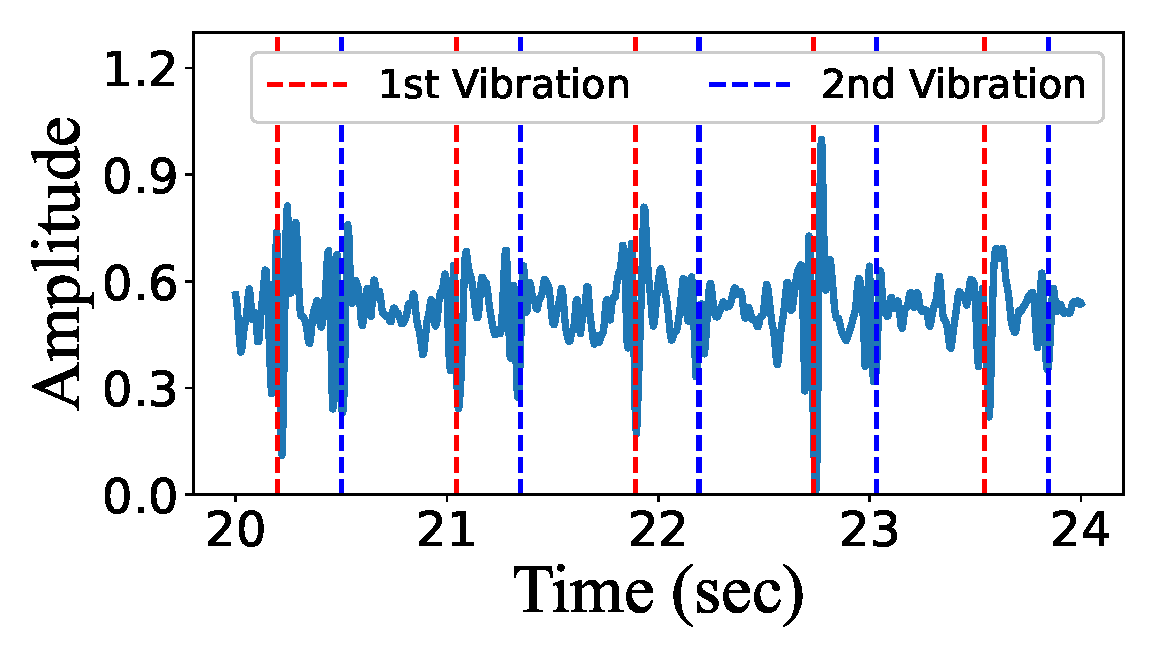
\includegraphics[width=0.25\columnwidth]{target_org.eps}}
  \subfloat[]{\label{fig:target_sig}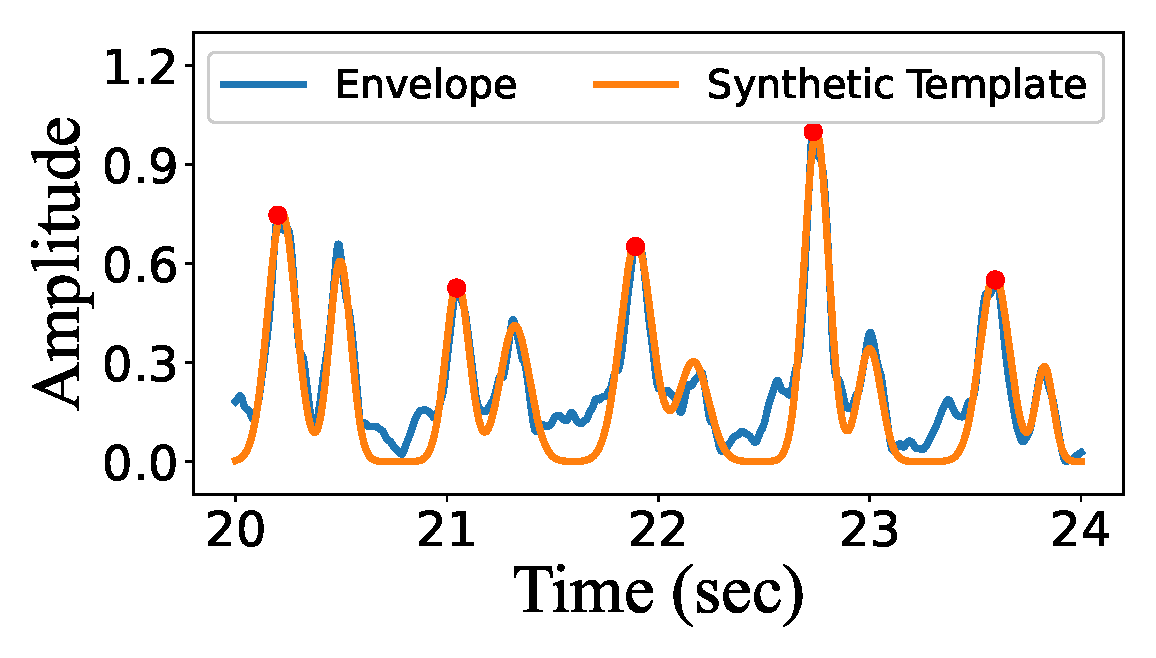
\includegraphics[width=0.25\columnwidth]{target_sig.eps}} 
  \subfloat[]{\label{fig:target_org_bad}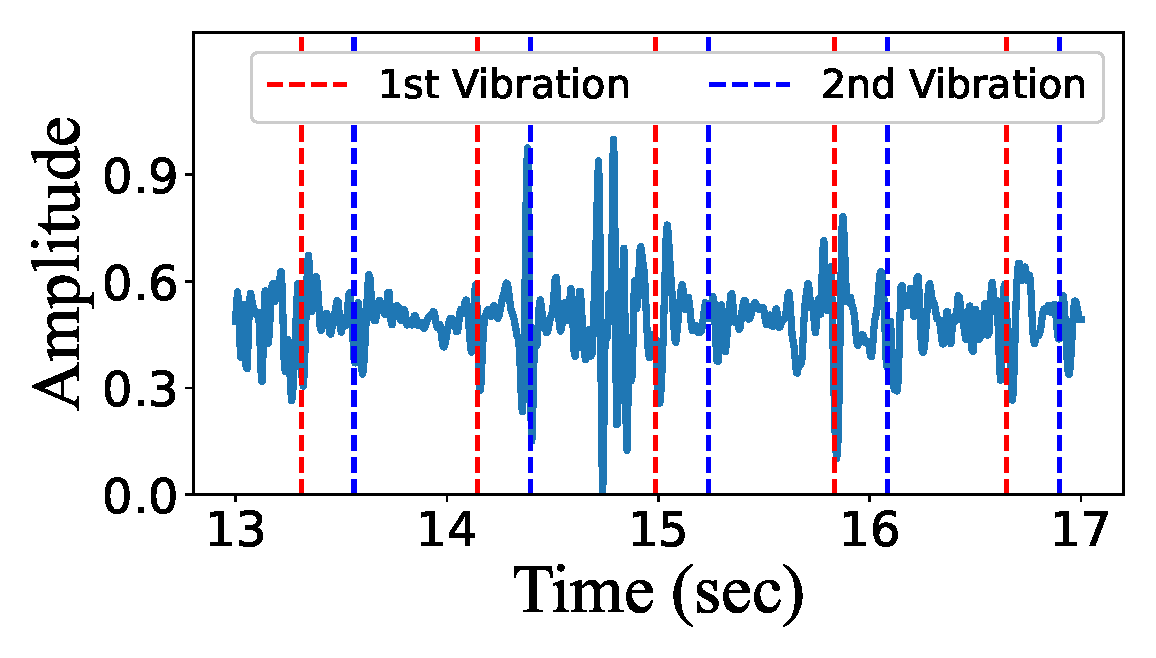
\includegraphics[width=0.25\columnwidth]{target_org_bad.eps}}
  \subfloat[]{\label{fig:target_sig_bad}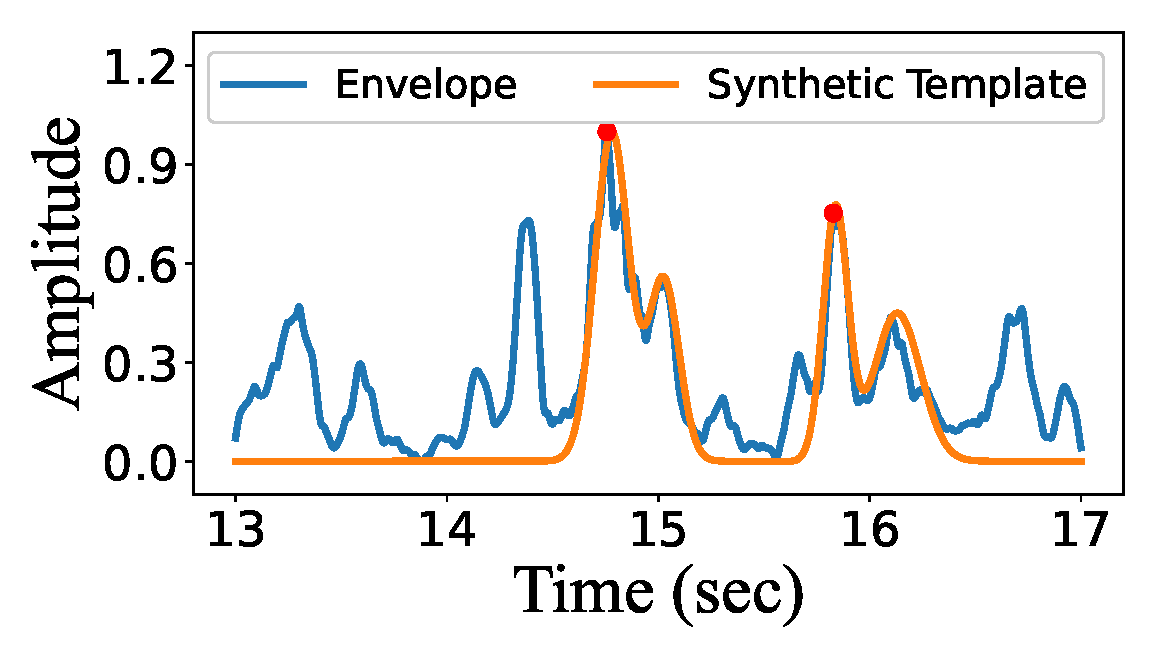
\includegraphics[width=0.25\columnwidth]{target_sig_bad.eps}}
  \caption{Template for assessing SNR: (a) High-SNR radar signal; (b) Extracted signal envelope with the synthetic template; (c) (a) Low-SNR radar signal, (d) Extracted signal envelope with the synthetic template.}
  \label{fig:template}
\end{figure}

\subsubsection{Derivative-free Optimization (DFO)}
The MSE values obtained from template matching for the radar pieces extracted from point $E$ will be used as costs $\mathcal{F}(E)$ in searching CF point, but the traditional gradient-based optimization method is not applicable because there is no explicit cost function. Therefore, the CFT algorithm is developed in a derivative-free manner based on coordinate search (CS) algorithm~\cite{larson2019derivative}, to asymptotically approach the CF point. 

The definition of the DFO problem is formulated as:
\begin{equation}
E_b = \underset{E \in \mathbb{R}^n}{\arg \min }\left\{\mathcal{F}(E) : E\in \Omega \right\}
\end{equation}
with $\Omega$ representing a user-defined constrained $n$-dimensional search space near initial point $E_0$ as shown in Figure~\ref{fig:CFTRFcardi}(b), and the cost of points out of the constraint will be set as $\mathcal{F}(E\not\in \Omega)=\infty$. During each iteration $k$, many trial points $E_k$ within the constraint will be evaluated to find the incumbent points $E_i$ as the temporary best point for the next iteration. 

To perform a derivative-free search, the traditional CS algorithm starts from the initialization of grids $G_k$:
\begin{equation}\label{equ:grid}
G_k := \{E_k + \gamma_kD\} \subset \mathbb{R}^n
\end{equation}
where $\gamma_k>0$ is the grid size parameter and $D$ contains several vectors $p$ for possible searching directions, as shown in Figure~\subref*{fig:cft_1}. The local convergence of CS is ensured by dense search directions $D$ and a refined grid size $\gamma_k$ to find better $E_i$ compared with current $E_k$~\cite{larson2019derivative}. However, the highly discontinuous objective space for radar-monitored vital signs may have numerous local minima that distract the optimization algorithm, i.e., the signal SNR of the adjacent points might be very different, as shown in Figure~\subref*{fig:radar_good} and~\subref*{fig:radar_bad}.

\begin{figure}[tb]
  \centering
  \subfloat[]{\label{fig:cft_1}\includegraphics[width=0.2\columnwidth]{cft_1.pdf}}\hspace{0.02\columnwidth}
  \subfloat[]{\label{fig:cft_2}\includegraphics[width=0.2\columnwidth]{cft_2.pdf}} \\
  \subfloat[]{\label{fig:cft_3}\includegraphics[width=0.35\columnwidth]{cft_3.pdf}}
  \caption{Illustration of the CFT algorithm with bold line wrapping the search region $S_k$: (a) Equality between $\gamma$ and $\Gamma$ (same as in CS algorithm); (b) Large $\Gamma_k$ with refined $\gamma_k$, providing more potential points to be evaluated; (c) Jump out of the local minimum by adjusting $\Gamma_k$ and $\gamma_k$.}
  \label{fig:cft_plot}
\end{figure}

To jump out of the potential local minimum, CFT algorithm is proposed by introducing search region $S_k$ to restrict the possible search directions $p$, alleviating the difficulty of searching in numerous dense grid points and allowing the adjustment of search region and grid size iteratively to break the local minimum. The detailed procedures of CFT are shown in Algorithm~\ref{alg:CFT}, with an illustration of $\mathbb{R}^2$ space shown in Figure~\ref{fig:cft_plot}. 

In CFT, the grids $G_k$ is still expressed as in (\ref{equ:grid}) and the newly introduced search region $S_k$ is expressed as:
\begin{equation}
S_k := \{E\in G_k : \| E-E_k \|_{\infty} \leq \Gamma_k a \}
\end{equation}
with $a=\max \left\{\left\|a^{\prime}\right\|_{\infty}: a^{\prime} \in D\right\}$ and $\Gamma_k$ as the size parameter for the search region. An intuitive interpretation of $S_k$ is the point set that contains grid points inside and on the boundary of the bold line controlled by $\Gamma_k$, as shown in Figure~\subref*{fig:cft_2}.

Based on the well-constructed grids $G_k$ and search region $S_k$, the remaining CFT algorithm is performed with searching and resizing stages:

\textbf{Searching: } The searching stage simply asks for the evaluation of $\mathcal{F}(E)$ on a subset of grids $G_k$ based on any sampling algorithm (e.g., Latin hypercube sampling~\cite{larson2019derivative}), as indicated in line~\ref{line:s1} in Algorithm~\ref{alg:CFT}.

\textbf{Resizing: } The resizing stage depends on the result of searching stage: 
\begin{itemize}
  \item If a new incumbent point $E_i$ is found with better SNR, the search region will be doubled as $\Gamma_{k+1}=2\Gamma_k$ (line~\ref{line:r1}), and the grid size will be empirically set as $\gamma_{k+1}=\min(\Gamma_k, {\Gamma_k}^2)$ (line~\ref{line:r4}), enabling to search in broader space in the next iteration.
  \item If there is no better point than the current $E_k$ on the current grids $G_k$, another searching stage will be performed only within the search region $S_k$ (line~\ref{line:s2}). Then, If a better point $E_i$ is found, $\Gamma_{k+1}$ and $\gamma_{k+1}$ is obtained as above (line~\ref{line:r2}), otherwise, the search region will be halved as $\Gamma_{k+1}=\Gamma_k/2$ (line~\ref{line:r3}) for a finer search with $\gamma_{k+1}=\min(\Gamma_k, {\Gamma_k}^2)$ (line~\ref{line:r4}).
\end{itemize}

The searching step enables the finding of better points $E_i$ in a broad space, and the resizing step either refines the grid if the current $\gamma_{k}$ is not enough or enlarges the search space when stalling at the local minimum, as shown in Figure~\subref*{fig:cft_3}. Finally, the CFT algorithm will be terminated after achieving a desired SNR$_d$ or iteration limit $k_{max}$.

\begin{algorithm}[tb]
\caption{CFT Algorithm}\label{alg:CFT}
\begin{algorithmic}[1]
    \State \textbf{Input:} $E_0$, SNR$_d$, $k_{max}$
    \State \textbf{Output:} $E_b$, SNR$_b$
    \Statex \textsc{Objective}:
    \State $E_b = \underset{E \in \mathbb{R}^n}{\arg \min }\left\{\mathcal{F}(E) : E\in \Omega \right\}$
    \State Initialize $k=0$, $\Gamma_k = \gamma_k = 1$, $SNR_b=\mathcal{F}(E_k)$
    \While {$SNR_b>SNR_d$ and $k<k_{max}$}
% \Statex \textsc{Searching}:
    \If{$\mathcal{F}(E)<SNR_b$ for some $E\in G_k$} \label{line:s1}
      \State $E_{k+1}\leftarrow E$, $SNR_b \leftarrow \mathcal{F}(E)$ 
      \State $\Gamma_{k+1}\leftarrow 2\Gamma_k$ \label{line:r1}
% \Statex \textsc{Resizing}:
% \Statex \textsc{Searching}:
    \ElsIf{$\mathcal{F}(E)<SNR_b$ for some $E\in S_k$} \label{line:s2}
% \Statex \textsc{Resizing}:
      \State $E_{k+1}\leftarrow E$, $SNR_b \leftarrow \mathcal{F}(E)$
      \State $\Gamma_{k+1}\leftarrow 2\Gamma_k$ \label{line:r2}
    \Else
      \State $E_{k+1} \leftarrow E_{k}$
      \State $\Gamma_{k+1}\leftarrow \Gamma_k/2$ \label{line:r3}
    \EndIf
    \State $\gamma_{k+1}\leftarrow \min(\Gamma_k, {\Gamma_k}^2)$ \label{line:r4}
    \State $k \leftarrow k+1$, $E_b \leftarrow E_{k+1}$
    \EndWhile
\end{algorithmic} 
\end{algorithm} 

The visualization of the CFT algorithm in Figure~\ref{fig:CFTRFcardi}(b) shows that initial iterations search in a large space, and the algorithm could jump out of the green local minima to find the red CF point within the fine blue grid points. In addition, the tracking of the CF points along time can be naturally realized by repeating Algorithm~\ref{alg:CFT} with previous $E_b$ as the new $E_0$, and the SNR evaluated on the previous point might have already achieved SNR$_d$ due to the quasi-static human body, saving a huge amount of time for calculating useless channel information for filtering or clustering~\cite{li2024radarnet,chen2022contactless,liu2024diversity}. 

\subsection{Transfer Learning for ECG Recovery}
\subsubsection{Deep Learning Model Design}
The radar signal extracted from the $10$ best points from CFT algorithm will be converted to spectrograms as the input for deep learning model according to our previous work~\cite{zhang2024radarODE-MTL}, providing extra frequency-domain information to assist model training. The deep learning model adopts the popular backbone-decoder structure as designed in~\cite{zhang2024radarODE-MTL}:
\begin{itemize}
  \item The backbone leverages ResNet~\cite{he2020resnet} framework with deformable 2D convolution layer~\cite{dai2017deformable} to efficiently extract cardiac features from image-like spectrogram inputs.
  \item The decoder is based on 1D convolutional neural network (CNN) to generate corresponding signals either for the pre-text task or ECG signal recovery. 
\end{itemize}

\subsubsection{Pre-text Task Training and Fine-tuning}
The pre-text task used for SSL should reveal certain inherent features in the radar-monitored vital sign, and two major features used for traditional heart rate estimation are periodicity and sparsity~\cite{zhang2023overview}. In this work, the duration of each segment is $4$ sec and may not reveal strong periodicity. Therefore, SSR will be used as the pre-text task in RFcardi and is defined as:
\begin{equation}
h=\Phi x+n
\end{equation}
where $h$ is the high-SNR radar signal, $\Phi$ means the observation matrix, $x$ is the sparse representation for heartbeats and $n$ represents the residual noise. The traditional SSR task can be seemly converted to a system identification problem by viewing $\Phi$ as a multi-channel adaptive filter, and the estimation of the filter coefficient is the same as training a CNN-based neural network (i.e., training CNN kernels)~\cite{ha2020contactless}.

In this case, the SSR task is realized by using the aforementioned CNN-based backbone-decoder structure with the loss function:
\begin{equation}\label{equ:sparse}
\mathcal{L} = \|x -x^{\prime} \|_2 + \underbrace{\lambda_s\frac{\|x\|_1 / \| x\|_2-1}{\sqrt{m}-1}}_{\text{sparse penalty}}
\end{equation}
where $m$ is the length of the signal, $x$ is the output the from deep learning model, $x^{\prime}$ is the sparse ground truth with values for the radar peaks maintained (1st vibration in Figure~\subref*{fig:target_org}) while other values are set to $0$. The sparse penalty has a range of $[0,\lambda_s)$ with a smaller value indicating better sparsity~\cite{hoyer2004non}.

After pre-training based on SSR, the parameters of backbone will be retained with a new decoder connected (same structure as for pre-text task training), and a few radar-ECG pairs are used for fine-tuning the pre-trained RFcardi model using MSE as the loss function.

\section{Details of Experiment and Dataset}\label{sec:exp}
\subsection{Experimental Details}\label{sec:data_coll}
\subsubsection{Dataset Collection and Preparation}
The dataset contains a total of $80$-minute synchronous radar-ECG pairs collected for $5$ healthy subjects ($3$ men, $2$ women) in $2$ indoor scenarios as shown in Figure~\ref{fig:data_col}. The subjects are asked to sit causally and are allowed to change postures during data collection, and each data trial lasts for $1$ minute. The distance between radar and human body varies from $0.5-1.2$m, and a longer distance causes the decrease of signal SNR with a smaller portion of the space points containing useful cardiac features. 

TI-AWR 1843 radar with $2$ Tx and $4$ Rx is used for data collection with $8$ virtual antenna channels created~\cite{AWR1843}, and the radar configurations are listed in Table~\ref{tab:data_param} with the name provided in TI mmWave-Studio interface. The signal will be sampled as $200$Hz, and only a band-pass filter from $0.5$ to $50$Hz and a differentiator are used for removing respiration noise because the radar signal extracted from CF points already has high SNR. Lastly, the ECG ground truth is collected using TI ADS1292, and the related ECG processing (e.g., smoothing and peak finding) is realized by NeuroKit2 python package~\cite{makowski2021neurokit2}.

\begin{figure}[tb]
  \centering
  \includegraphics[width=0.6\columnwidth]{scen_1.pdf}
  \caption{Indoor scenarios for data collection.}
  \label{fig:data_col}
\end{figure}

\begin{table}[tb]
\centering
\caption{Parameters for data collection interface}
    \begin{tabular}{lc?lc}
    \toprule
    \textbf{Parameter} & \textbf{Value} & \textbf{Parameter} & \textbf{Value} \\
    \toprule
    Start Frequency & $77$GHz & Frequency Slope & $65$MHz/$\mu$s \\ 
    Idle Time & $10\mu$s    & Tx Start Time & $1\mu$s \\
    ADC Start Time & $6\mu$s  & ADC Samples & $256$ \\ 
    Sample Rate & $5000$kbps  & Ramp End Time & $60\mu$s \\ 
    % Rx Gain & $30$ dB  & Rx Gain Target & $30$ dB  \\ 
    Start/End Chirp Tx & $0/2$  & No. of Chirp Loops & $2$  \\ 
    No. of Frames & $12000$  & Frame Periodicity & $5$ms  \\ 
    \bottomrule
    \end{tabular}
\label{tab:data_param}
\end{table}%

\subsection{Implementation Details}
\subsubsection{Parameters for CFT Algorithm}
The constraint $\Omega$ for the CF point search is centered at the initial state $E_0$ with a range of $0.4\times 0.2 \times 0.4$m as illustrated in Figure~\ref{fig:CFTRFcardi}(b). In addition, the initial grid and search region size should be adjusted to fit the real-life physical unit as $\Gamma_k= \gamma_k = 0.1$m, and the size will be limited as $\Gamma_k\geq\gamma_k\geq 0.001$m to prevent an exhaustive search within a meaningless small space. At last, SNR$_d$ is set to $0.01$ for the desired MSE between normalized synthetic template and signal envelope, and $k_{max}$ is set to $100$.

\subsubsection{Deep Learning Model Training}
The deep learning model adopts the same backbone, ECG decoder and hyperparameters as in our previous open-sourced work~\cite{zhang2024radarODE-MTL} coded in PyTorch and trained on NVIDIA RTX 4090 (24GB). The total training epoch is set to $100$ with batch size $8$, and a $5$-fold cross-validation training strategy is adopted to split the dataset to make the most of the limited dataset while excluding the testing data from the training phase. The parameter for balancing the weight of sparse penalty is set as $\lambda_s=0.1$.


\subsection{Methods for Comparison}
The comparison is performed with the representative methods based on accumulation and clustering to extract high-SNR radar signal:
\begin{itemize}
  \item De-ViMo~\cite{liu2024diversity} is proposed for heart rate monitoring and is based on the accumulation of signals from various dimensions (e.g., chirps, antennas, spatial points) to enhance cardiac features while mitigating noise. In addition, De-ViMo also improves the rough localization by identifying the peaks in micro-motion frequency bands instead of the entire FMCW bands.
  \item MMECG~\cite{chen2022contactless} requires the calculation of numerous points in 3D space and applies clustering algorithm to improve SNR. Then, a pattern-matching process is performed to learn the common pattern from the clustered result and select the best radar signal(s).
\end{itemize}
In addition, to the best of our knowledge, this is the first paper that leverages SSL with an appropriate pre-text task for pre-training of radar-based ECG recovery, and only the performance analysis will be provided without comparison with other methods.

\begin{figure*}[tbp]
  \centering
  \begin{minipage}{0.1\linewidth}\centering
\rotatebox[origin=center]{0}{\textbf{Rough Loc.}}
\rotatebox[origin=center]{0}{$\approx$}\\
\rotatebox[origin=center]{0}{\textbf{CF Point}}
\end{minipage}\begin{minipage}{0.9\linewidth}\centering
  \subfloat[]{\label{fig:bf_good}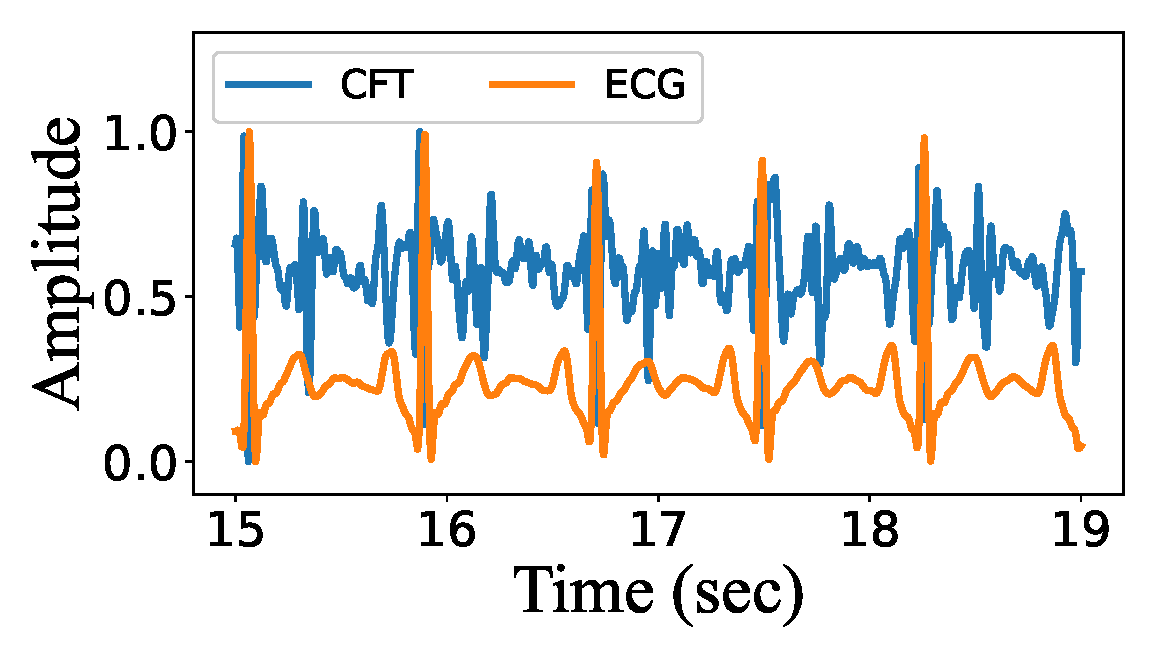
\includegraphics[width=0.3\columnwidth]{bf_good.eps}}
  \subfloat[]{\label{fig:MMECG_good}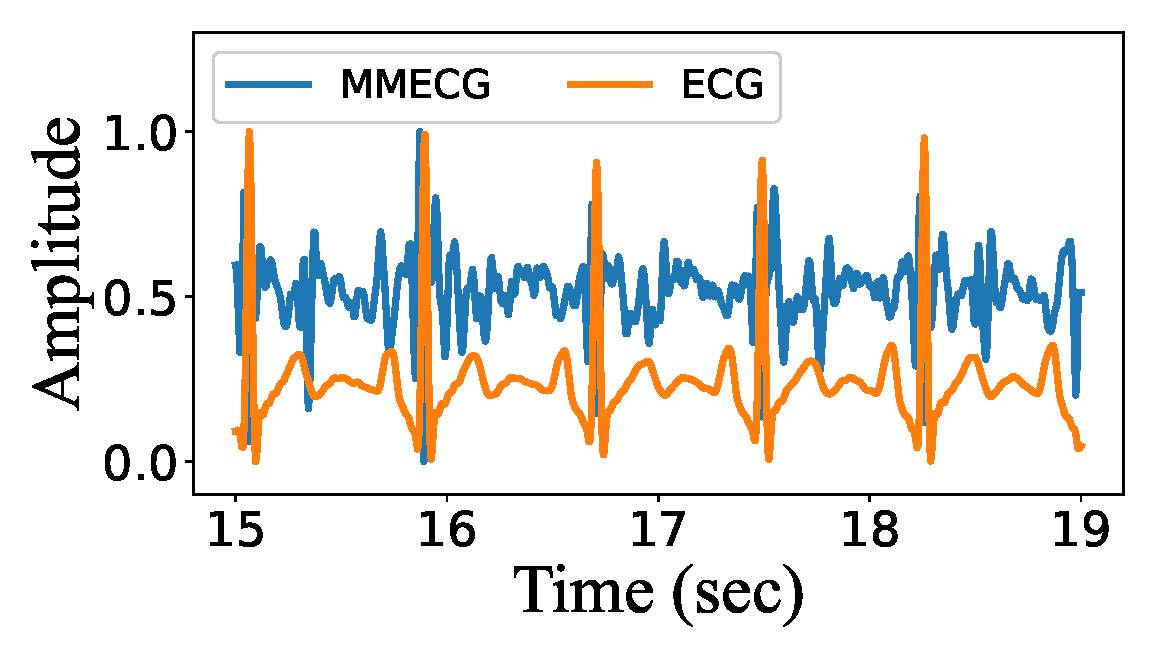
\includegraphics[width=0.3\columnwidth]{mmecg_good.eps}}
  \subfloat[]{\label{fig:vimo_good}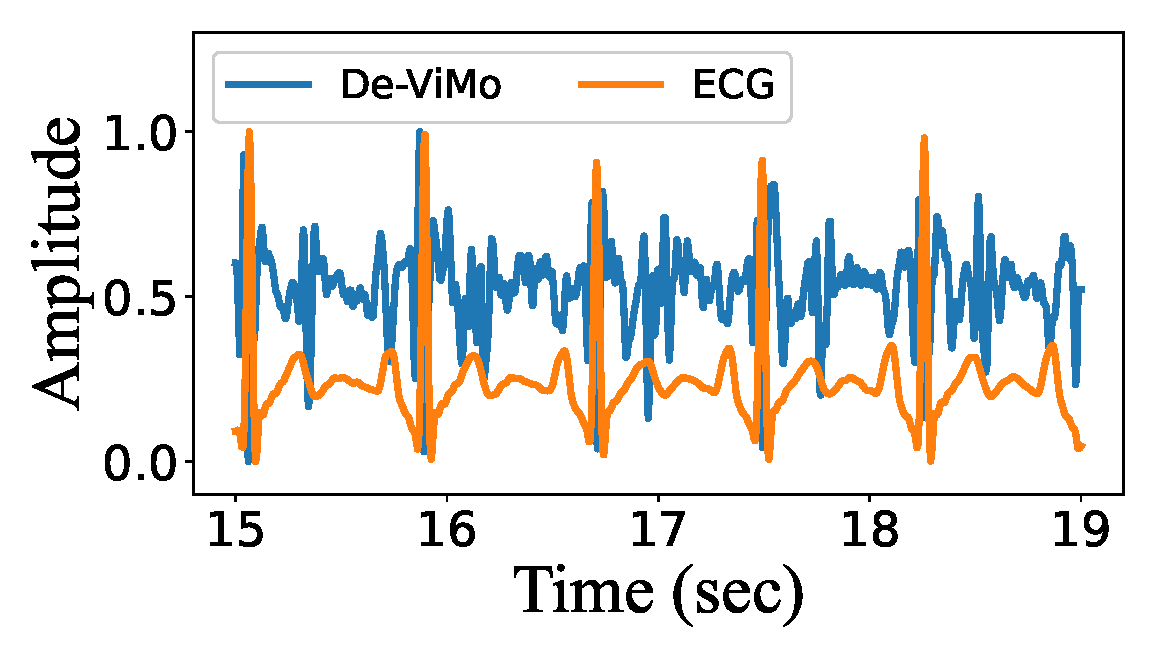
\includegraphics[width=0.3\columnwidth]{devimo_good.eps}}\\
\end{minipage}
\begin{minipage}{0.1\linewidth}\centering
\rotatebox[origin=center]{0}{\textbf{Rough Loc.}}
\rotatebox[origin=center]{0}{$\neq$}\\
\rotatebox[origin=center]{0}{\textbf{CF Point}}
\end{minipage}\begin{minipage}{0.9\linewidth}\centering
  \subfloat[]{\label{fig:bf_bad}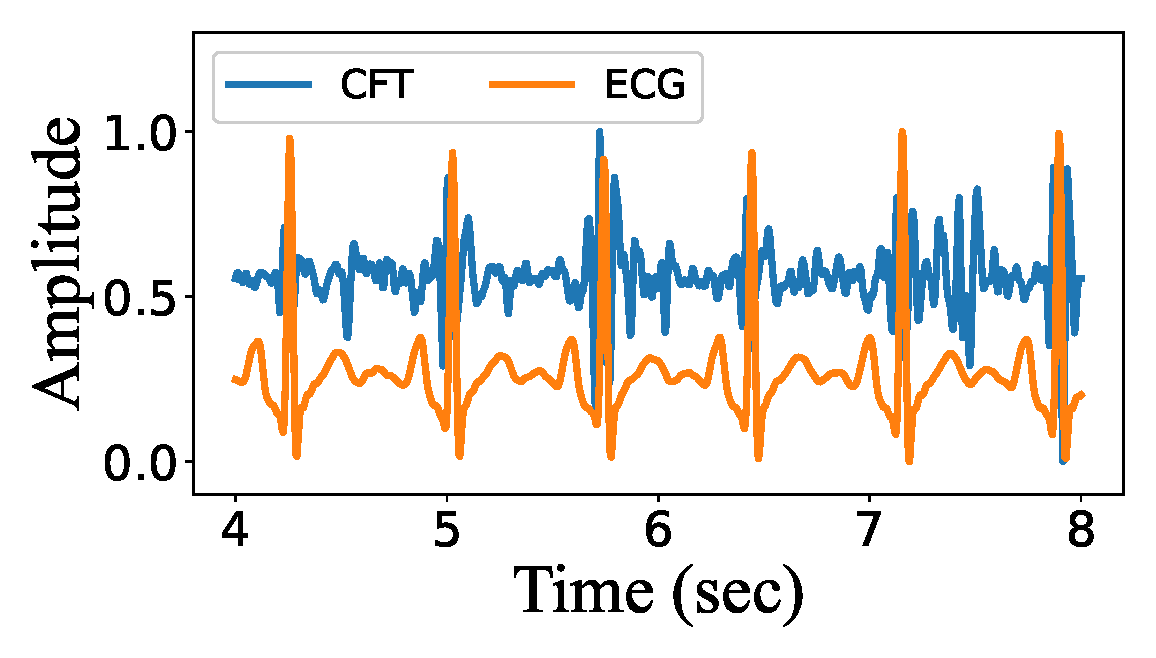
\includegraphics[width=0.3\columnwidth]{bf_bad.eps}}
  \subfloat[]{\label{fig:MMECG_bad}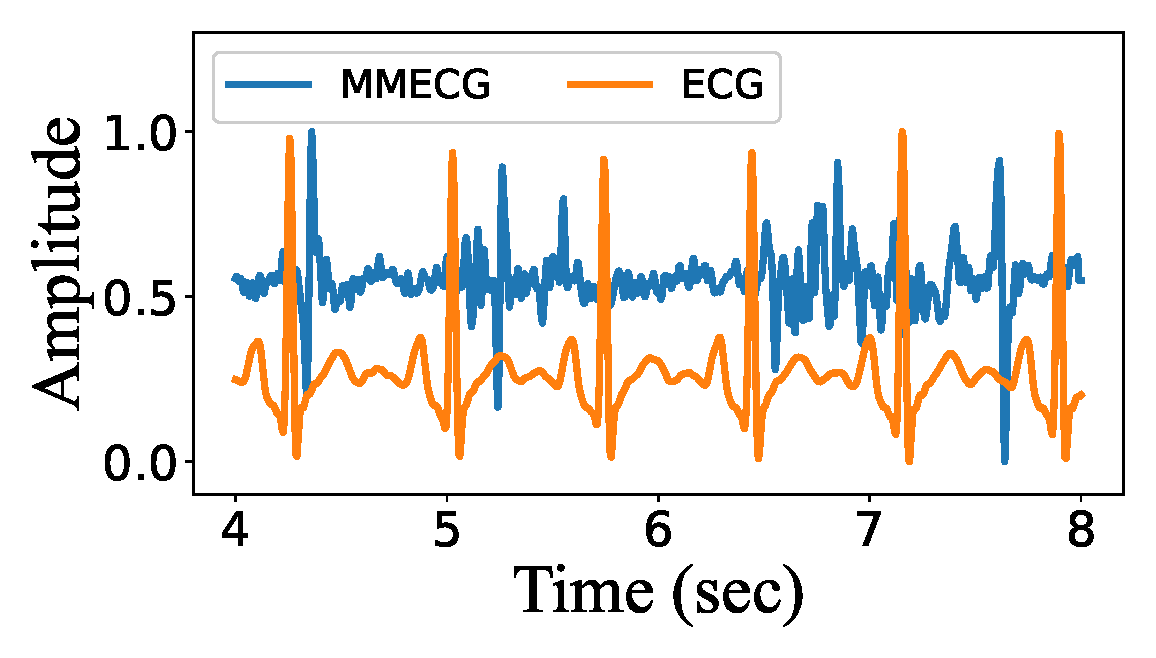
\includegraphics[width=0.3\columnwidth]{mmecg_bad.eps}}
  \subfloat[]{\label{fig:vimo_bad}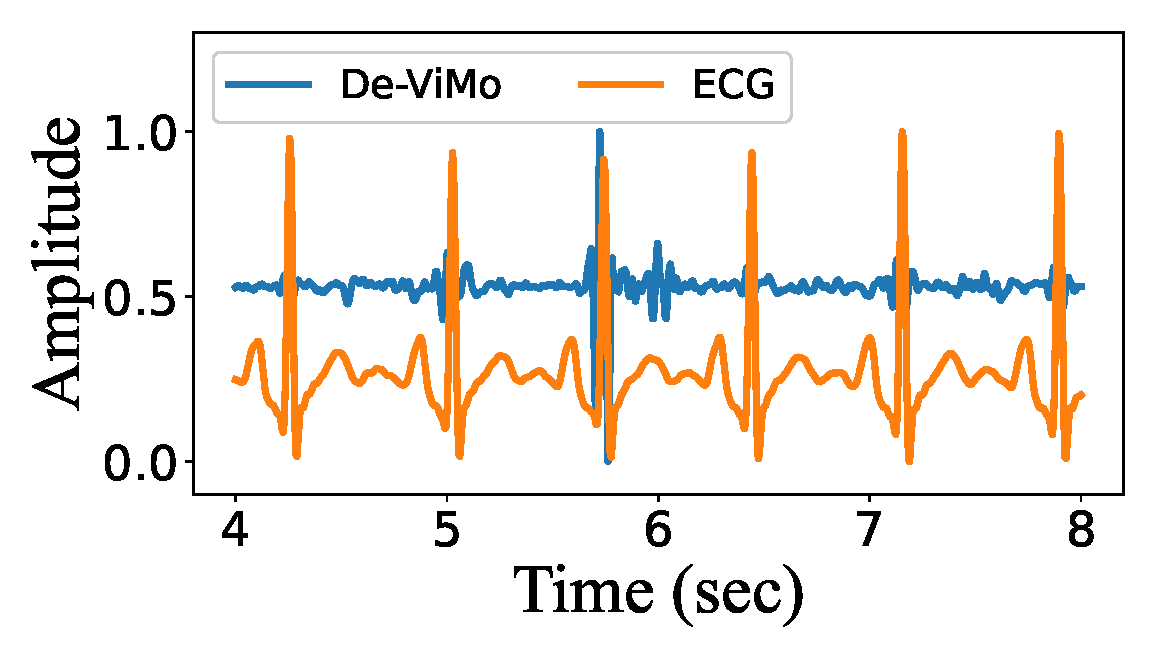
\includegraphics[width=0.3\columnwidth]{devimo_bad.eps}}
\end{minipage}
  \caption{Visualization of the extracted radar signal for all methods: (a) - (c) If CF point is around rough body location; (d) - (f) If CF point is far from rough body location.}
  \label{fig:compare_overall}
\end{figure*}

\section{Experimental Results and Evaluations}\label{sec:result}
\subsection{Performance of CFT Algorithm}
\subsubsection{Effectiveness of CFT Algorithm}
The examples of the extracted radar signal for different methods are shown in Figure~\ref{fig:compare_overall}, illustrating that precise cardiac localization has a huge effect on the signal quality. For example, if the rough body location is around CF point, all three methods can obtain high-SNR signals with clear first and second vibrations using either space search (CFT, Figure~\subref*{fig:bf_good}), clustering (MMECG, Figure~\subref*{fig:MMECG_good}) or accumulation (De-ViMo, Figure~\subref*{fig:vimo_good}). 

In contrast, only a few range bins will contain useful cardiac features if the rough body location is far from CF points, especially when increasing the monitoring range. Therefore, the signal accumulation may enhance the noises as shown in Figure~\subref*{fig:vimo_bad} while the signal clustering may also encounter a failure due to the lack of homogeneous cardiac signals as shown in Figure~\subref*{fig:MMECG_bad}. However, The proposed CFT could precisely locate the CF point with good SNR subject to the designed signal template and DFO searching strategy, and the extracted radar signal still shows clear peaks as shown in Figure~\subref*{fig:bf_bad}.

During the data collection of this study, the subjects are allowed to change postures to alleviate discomfort, with a resultant CF point deviation of several decimeters, while the rough location provided by FMCW signal processing is still unchanged. Therefore, the proposed CFT algorithm is essential because the posture change is inevitable, and a thorough evaluation in terms of different monitoring ranges will be performed in the next part.

\subsubsection{Impact of Monitoring Range}
To evaluate the performance of different methods when increasing the monitoring range, the quality of extracted radar signals for all trials is evaluated in terms of:
\begin{itemize}
\item Absolute Peak error between ECG R peaks and the dominant peaks for the first vibrations in radar signal.
\item Missed detection rate (MDR) to count the cardiac cycles with no peak detected or with the absolute peak error larger than $150$ms~\cite{chen2022contactless}.
\end{itemize}

Figure~\subref*{fig:pk_err_point} and~\subref*{fig:pk_mdr_point} illustrate the peak error and MDR for all $80$ trials with corresponding fitting curves indicating the mean peak error or MDR. All the methods show similar performance in the short range and experience certain degradation with respect to the increasing range. In particular, MMECG shows larger degradation and variance for longer-range cases because the rough localization based on FMCW signal processing cannot provide accurate cardiac location, and the resultant evaluated points may not capture useful information for clustering. In contrast, De-ViMo could provide a better cardiac location, and the accumulated results show better accuracy than MMECG, while the long-range monitoring still affects the quality because the accumulation is not robust to non-gaussian noise. At last, the proposed CFT could precisely focus on the CF point and keep tracking the high-SNR points during data collection, providing the best results with small variance for both peak error and MDR. 

\begin{figure}[tb]
  \centering
  \subfloat[]{\label{fig:pk_err_point}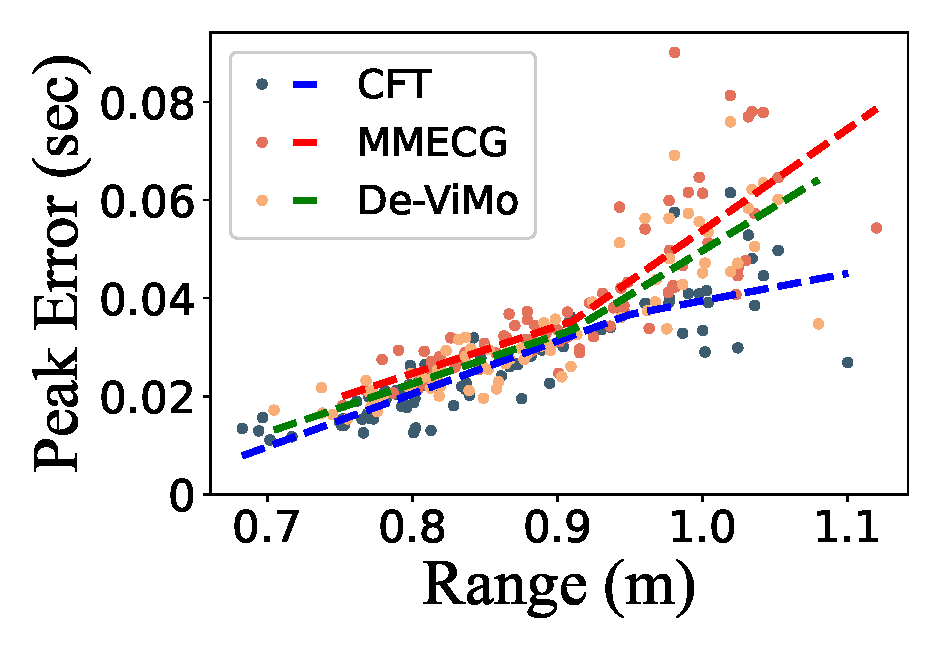
\includegraphics[width=0.4\columnwidth]{pk_err_point.eps}}
  \subfloat[]{\label{fig:pk_mdr_point}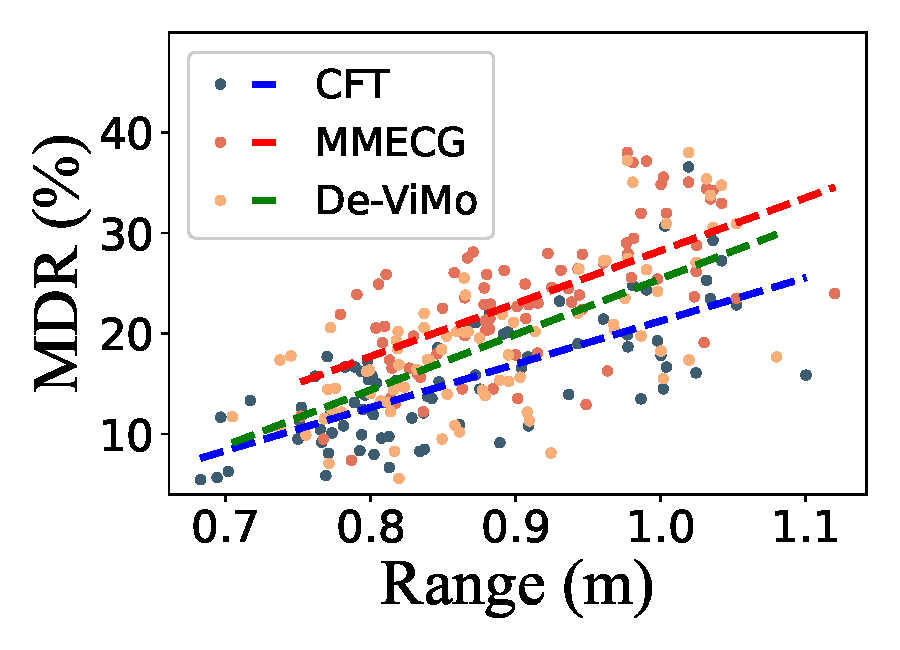
\includegraphics[width=0.39\columnwidth]{pk_mdr_point.eps}} \\
  \subfloat[]{\label{fig:pk_err_cdf}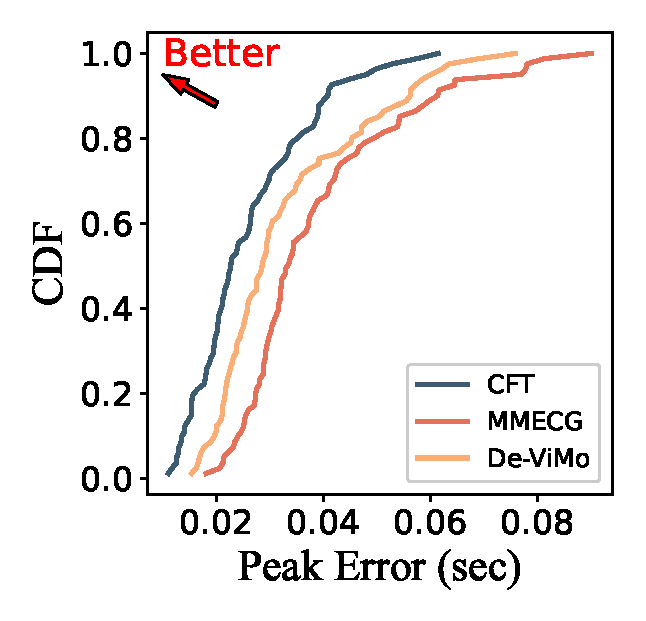
\includegraphics[width=0.4\columnwidth]{pk_err_cdf.eps}}
  \subfloat[]{\label{fig:pk_mdr_cdf}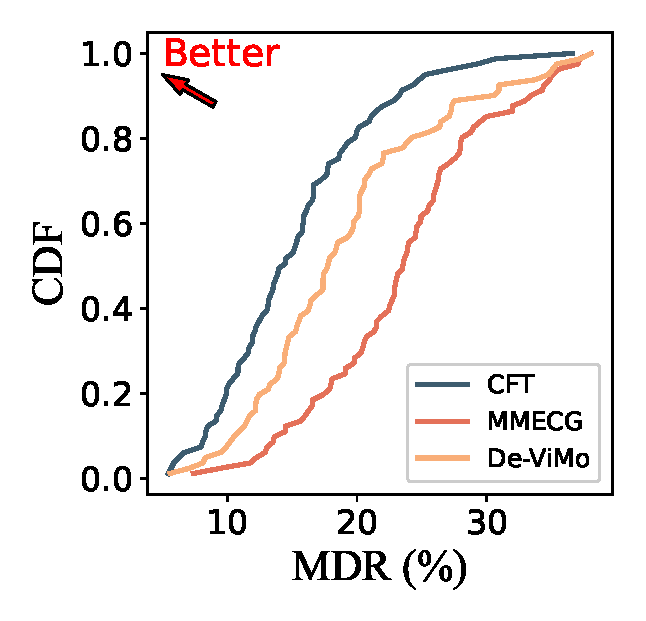
\includegraphics[width=0.4\columnwidth]{pk_mdr_cdf.eps}} 
  \caption{Illustration of performance in terms of peak error and MDR: (a) - (b) Scattered points with fitting curves along range axis; (c) - (d) CDF plots for all trails.}
  \label{fig:range_impact}
\end{figure}

In addition, the cumulative distribution function (CDF) plots for all trials are shown in Figure~\subref*{fig:pk_err_cdf} and~\subref*{fig:pk_mdr_cdf}. The proposed CFT algorithm achieves the best peak error with a median value of $0.022$~sec, while DE-ViMo and MMECG have worse performances with larger median values of $0.028$~sec and $0.033$~sec, respectively. Similarly, the precise localization and tracking of CF point also reduces the MDR for CFT results with a median value of $14\%$, while DE-ViMo and MMECG may affected by the accumulated noise or inaccurate cardiac localization with the median MDR of $17\%$ and $23\%$, respectively.

\begin{table}[tb]
\centering
\caption{Performance of supervised ECG recovery}
    \begin{tabular}{c |cccc}
    \toprule
    Methods  & \makecell[c]{MSE\\($\times 10^{-2}$)} $\downarrow$ & PCC $\uparrow$ & \makecell[c]{Peak Error \\ (ms)} $\downarrow$ & MDR $\downarrow$ \\
    \toprule
    MMECG~\cite{chen2022contactless} & $0.93$  & $80.36\%$ & $9.74$ & $7.96\%$ \\
    De-ViMo~\cite{liu2024diversity} & $0.88$ & $83.83\%$ & $8.93$ & $7.32\%$\\
    \midrule
    CFT  &  $\mathbf{0.82}$ & $\mathbf{85.47\%}$ & $\mathbf{7.61}$ & $\mathbf{6.85\%}$\\
    \bottomrule
    \end{tabular}%
\label{tab:ecg_supervise}
\end{table}%
\subsubsection{Impact of Signal Quality on ECG Recovery}
The signals extracted using different methods are used for supervised training to verify the impact of different input qualities on the ECG recovery task. The quality of the recovered ECG signal is assessed in terms of:
\begin{itemize}
\item The morphological accuracy is measured using MSE and Pearson-correlation coefficient (PCC), with MSE sensitive to the peak deviation and PCC focusing on the similarity between the ECG patterns.
\item The accurate recovery of ECG R peaks is crucial to coarse cardiac features calculation (e.g., heart rate variability) and is measured by absolute R peak error and MDR.
\end{itemize}
Table~\ref{tab:ecg_supervise} shows the performance of the deep learning model trained with datasets yielded by different methods. The training based on CFT dataset achieves the best results on both morphological accuracy (MSE$=0.0082$ and PCC$=85.47\%$) and R peak recovery (Peak Error$=7.61$ms and MDR$=6.85\%$), because the high-SNR inputs provide accurate peak locations with minor noise that affects the ECG pattern generation, as shown in Figure~\subref*{fig:radar_clean} and~\subref*{fig:ecg_pred_clean}. 

In contrast, MMECG and De-ViMo cannot preserve the signal quality especially for long-distance cases, and the noisy inputs will prevent the deep learning mode from identifying the accurate position of ECG pieces, causing large peak error and MDR, as shown in Figure~\subref*{fig:radar_noise} and~\subref*{fig:ecg_pred_noise}. It is worth noticing that poor signal SNR causes more degradation in peak error than morphological accuracy, because the ECG patterns share a similar shape and can be learned from other cardiac cycles, while the peak recovery (detection) fully relies on the current radar input and can be ruined by noises.

\begin{figure}[tb]
  \centering
  \subfloat[]{\label{fig:radar_clean}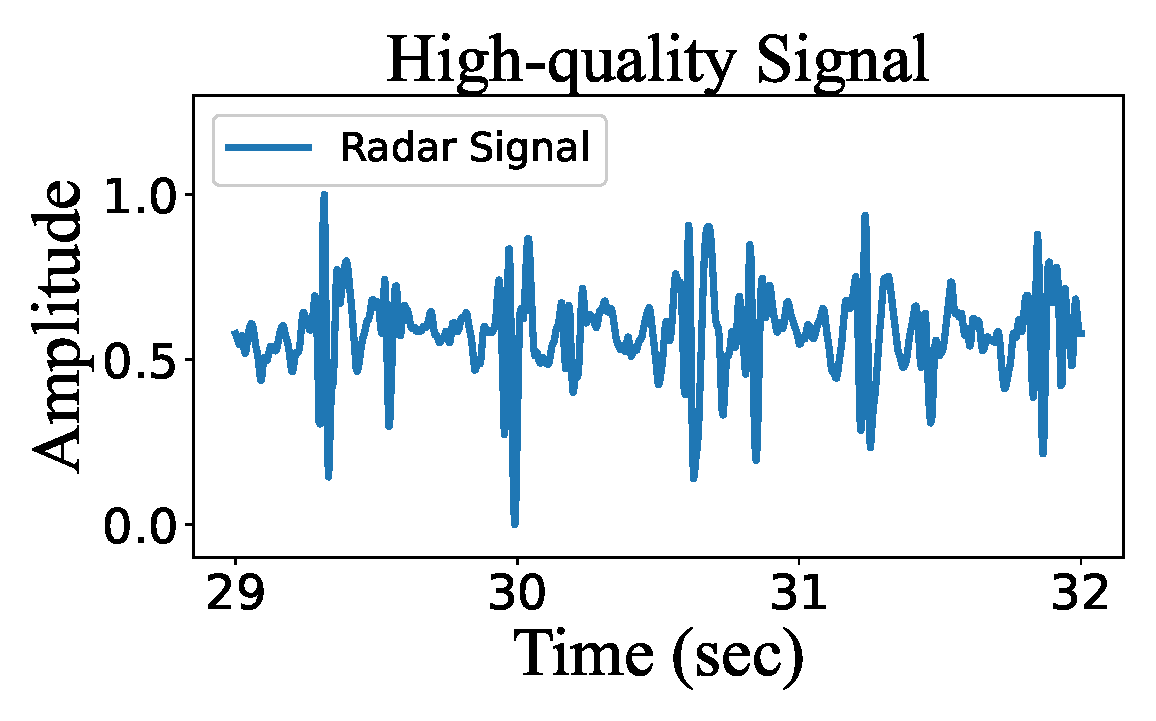
\includegraphics[width=0.25\columnwidth]{radar_clean.eps}}
  \subfloat[]{\label{fig:ecg_pred_clean}\includegraphics[width=0.25\columnwidth]{ecg_pred_clean.eps}} \\
  \subfloat[]{\label{fig:radar_noise}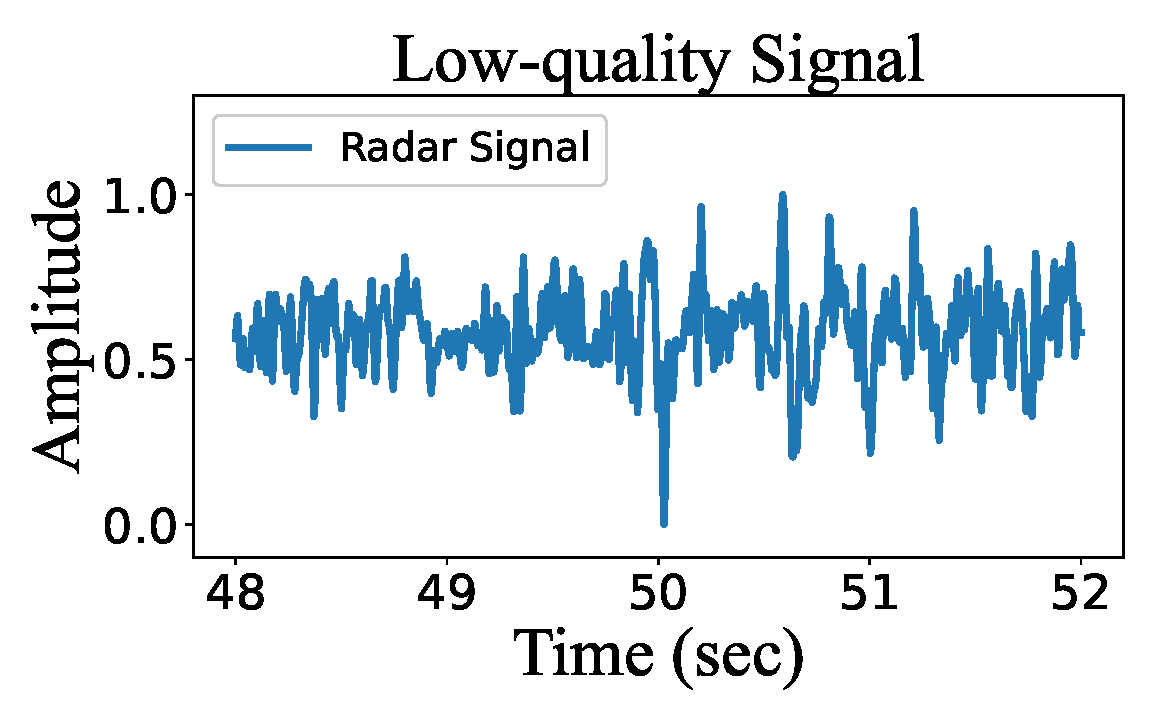
\includegraphics[width=0.25\columnwidth]{radar_noise.eps}}
  \subfloat[]{\label{fig:ecg_pred_noise}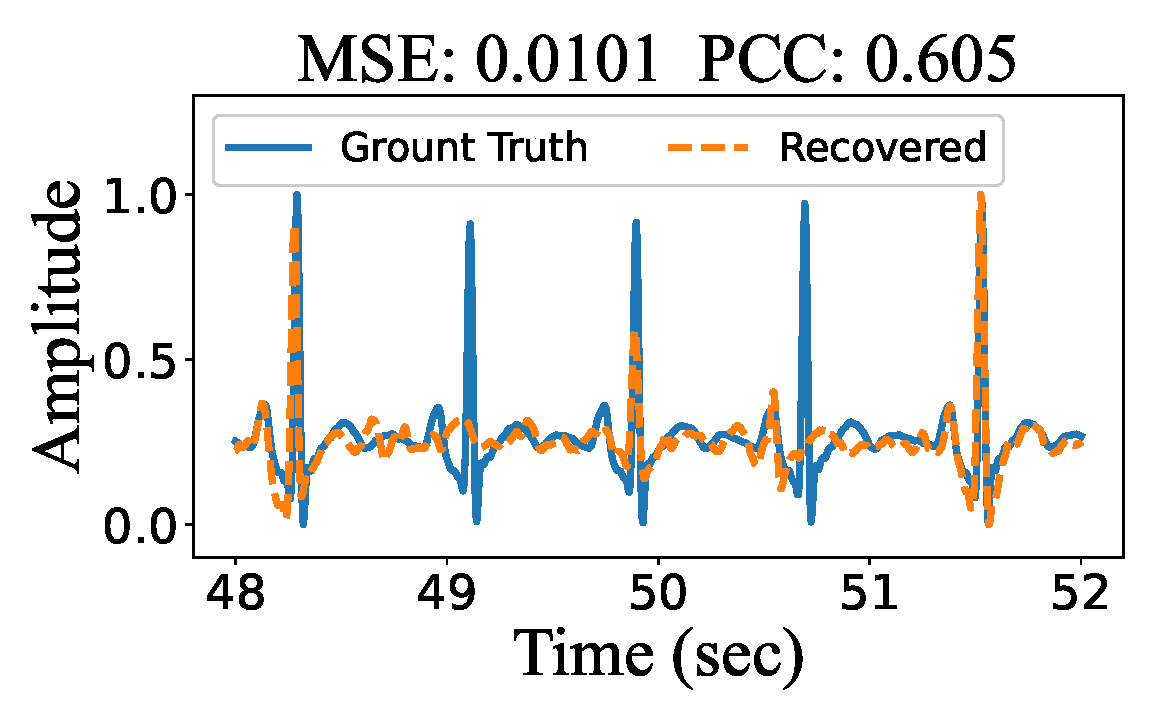
\includegraphics[width=0.25\columnwidth]{ecg_pred_noise.eps}} 
  \caption{Impact of radar input quality on the final ECG recovery: (a) - (b) High-quality radar input and ECG recovery; (c) - (d) Low-quality radar input and ECG recovery.}
  \label{fig:ecg_recovery}
\end{figure}
\begin{table}[tb]
\centering
\caption{Performance of SSL with ablation study}
    \begin{tabular}{c|cc?cc}
    \toprule
    {Methods} & \makecell[c]{MSE \\ ($\times 10^2$)} $\downarrow$ & Sparsity $\downarrow$ & \makecell[c]{MSE \\($\times 10^2$)} $\downarrow$ & Sparsity $\downarrow$ \\
    \midrule
    & \multicolumn{2}{c?}{\textbf{$\mathbf{100\%}$ Dataset}} & \multicolumn{2}{c}{\textbf{$\mathbf{80\%}$ Dataset}}  \\
    \midrule
    SSL w/o sp$^*$ & $0.91$ & $0.36$  & $0.96$ & $0.41$ \\
    SSL with sp    & $0.82$ & $0.20$  & $0.85$ & $0.22$ \\
    \midrule
    & \multicolumn{2}{c?}{\textbf{$\mathbf{60\%}$ Dataset}} & \multicolumn{2}{c}{\textbf{$\mathbf{40\%}$ Dataset}} \\
    \midrule
    SSL w/o sp & $1.43$ & $0.44$  & \multicolumn{2}{c}{Failed}\\
    SSL with sp    & $0.92$  & $0.26$  & $0.98$  & $0.31$\\
    \bottomrule
    \multicolumn{5}{l}{$^*$sp for sparse penalty}
    \end{tabular}%
\label{tab:ssr}
\end{table}%
\begin{figure}[tb]
  \centering
  \subfloat[]{\label{fig:ssr_bad}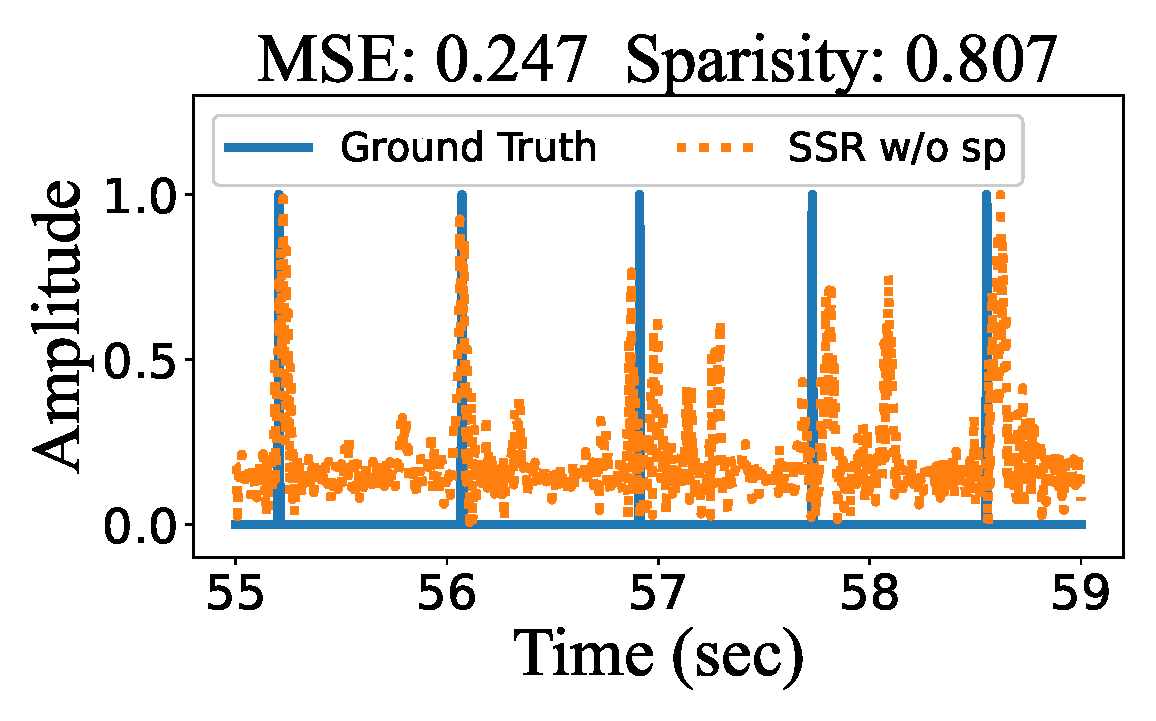
\includegraphics[width=0.4\columnwidth]{ssr_bad.eps}}
  \subfloat[]{\label{fig:ssr_good}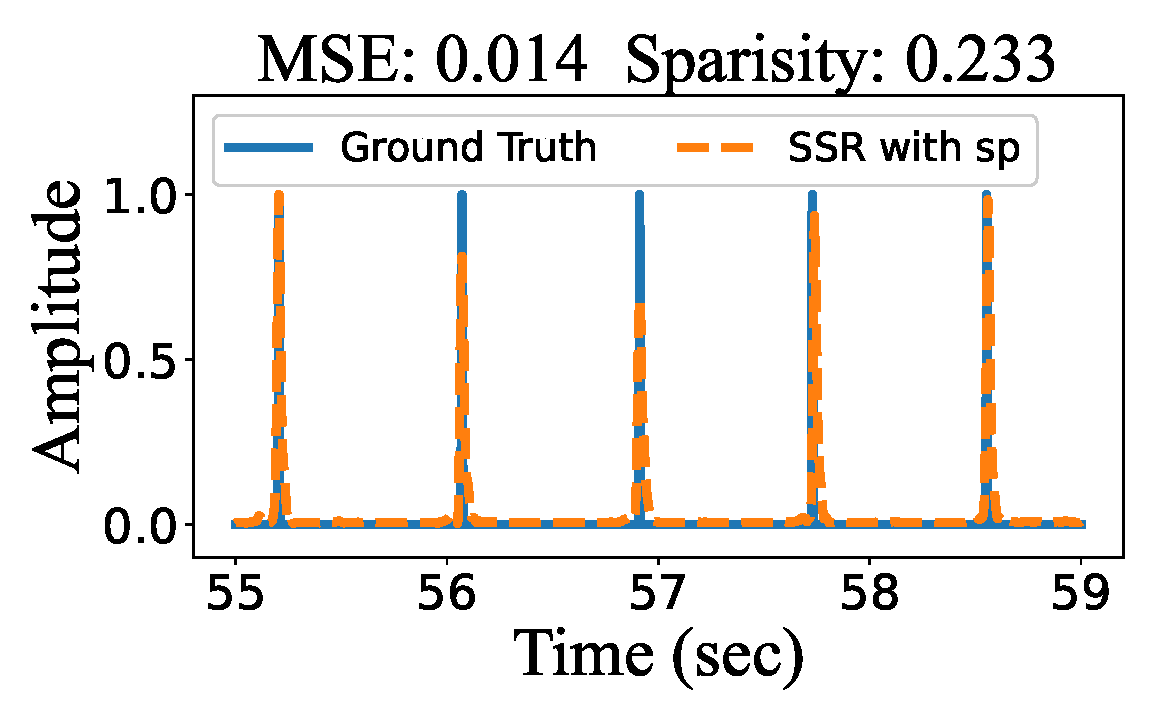
\includegraphics[width=0.4\columnwidth]{ssr_good.eps}}
  \caption{Results of SSR: (a) Failed SSR due to lack of data and sparse penalty; (b) Ideal SSR result with good MSE and sparsity.}
  \label{fig:ssr_res}
\end{figure}
\subsection{Performance of ECG Recovery using Transfer Learning}
\subsubsection{Evaluations and Ablation Studies of SSL}
The SSR task is crucial in the proposed transfer learning framework to provide latent representation that assists the further ECG pattern recovery, reducing the demand for radar-ECG pairs in the fine-tuning stage. The results of SSL are shown in Table~\ref{tab:ssr} in terms of MSE and sparsity to illustrate the former and latter part (without $\lambda_s$) in the loss function (\ref{equ:sparse}) for SSL training.

The experiment is repeated for different dataset scales with the ablation study on the use of sparse penalty, and the results indicate that both MSE and sparsity decrease with the reducing training data as shown in Table~\ref{tab:ssr}. Training with $100\%$ or $80\%$ dataset could achieve convergence and realize a successful SSR with similar MSE ($0.91, 0.82$) or ($0.96, 0.85$). However, the performance of SSR degrades heavily when further decreasing the training data without the constraint of sparse penalty, because the SSR results might fluctuate, as shown in Figure~\subref*{fig:ssr_bad}. In contrast, introducing the sparse penalty could suppress the fluctuation and force the deep learning model to focus only on the dominant peaks of the input radar signals, as shown in Figure~\subref*{fig:ssr_good}. Therefore, the training with sparse penalty loss still achieves good results with an MSE of $0.92$ and $0.98$ by using $60\%$ and $40\%$ of the dataset, while the model cannot be well-trained without sparse penalty by using $40\%$ dataset as shown in Table~\ref{tab:ssr} and Figure~\subref*{fig:ssr_bad}.

\subsubsection{Evaluations of Fine-tuning Results}
The fine-tuning is based on the model pre-trained by $100\%$ dataset with or without sparse penalty, and the experiment is repeated for different percentages of labeled data (i.e., radar signal with ECG ground truth). In addition, the same deep-learning model will be trained in a supervised manner by using the same amount of labeled data as the reference for transfer-learning ECG recovery. At last, an overall improvement will be provided by calculating the percentage of improvement across all four metrics to provide straightforward evaluations for different methods, as shown in Table~\ref{tab:ecg_few_shot}.

The fine-tuning with $100\%$ labeled data provides very similar performance in morphological accuracy with the MSE and PCC around $0.0080$ and $85.47\%$. It is worth noticing that the peak error and MDR are slightly improved, because the pre-text task SSR for pre-training is equivalent to identifying the peak position of the radar signal, and the learned representations can be seemly transferred to improve the accuracy of the recovered ECG R peaks, contributing to the overall improvement for transfer learning ($3.66\%$ and $1.75\%$).

Reducing $20\%$ of labeled data causes a $10\%$ overall degradation as shown in Table~\ref{tab:ecg_few_shot}, and the decline of peak error and MDR is more than MSE and PCC. The reason is that ECG morphological patterns for different cardiac cycles are similar and can be well-learned from $80\%$ labeled data with good MSE and PCC ($0.0084$ and $84.60\%$), while the location of each ECG piece is random and can be distorted by noises, requiring more training data for convergence.

The supervised training with $60\%$ labeled data cannot ensure a good morphological and peak accuracy and the overall degradation is $23.37\%$, with the PCC drop below $80\%$ as shown in Table~\ref{tab:ecg_few_shot}. In contrast, the pre-trained model still provided good results with mild degradations of $8.71\%$ and $12.68\%$. It is noticed that the effectiveness of sparse penalty in the SSL stage also affects the fine-tuning stage, because both peak error and MDR for transfer learning with spare penalty are better than those without sparse penalty, causing a large gap in the overall improvement compared with the previous training with $100\%$ and $80\%$ dataset.

Lastly, the deep learning model can barely learn from $40\%$ labeled dataset and yield a bad morphological and peak accuracy for supervised learning. In addition, examples of the recovered ECG for transfer learning with or without sparse penalty are shown in Figure~\ref{fig:fs_res}, and it is clear that the deep learning model struggles to learn both morphological and peak features from limited data if the pre-text task is not well-trained without sparse penalty, while Figure~\subref*{fig:fs_good} shows the good recovery because the pre-trained model transfer the learned representations from radar inputs to ECG recovery.


\begin{table}[tb]
\centering
\caption{Performance of ECG Recovery using different percentages of labeled data}
    \begin{tabular}{c |cccc|ccccc|c}
    \toprule
    {Methods} & \makecell[c]{MSE\\($\times 10^{-2}$)} $\downarrow$ & PCC $\uparrow$ & \makecell[c]{Peak Error \\ (ms)} $\downarrow$ & MDR $\downarrow$ & Overall $\uparrow$ & \makecell[c]{MSE\\($\times 10^{-2}$)} $\downarrow$ & PCC $\uparrow$ & \makecell[c]{Peak Error \\ (ms)} $\downarrow$ & MDR $\downarrow$  & Overall $\uparrow$\\
    \toprule
    &\multicolumn{5}{c}{\textbf{$\mathbf{100\%}$ Labeled}} & \multicolumn{5}{c}{\textbf{$\mathbf{80\%}$ Labeled}} \\ 
    \midrule
    Supervised & ${0.80}$ & ${85.47\%}$ & ${7.61}$ & ${6.85\%}$ & $0.00\%$ & $0.84$ & $84.60\%$ & $8.90$ & $8.04\%$ & $-10.09\%$ \\
    {TF w/o sp$^*$} & $0.81$ & $85.35\%$ & $8.46$ & $5.51\%$ & $1.75\%$ & $0.82$ & $86.36\%$ & $8.35$ & $7.02\%$ & $-3.42\%$ \\
    {TF with sp} & $0.80$ & $85.51\%$ & $8.40$ & $5.14\%$ & $3.66\%$ & $0.81$ & $84.29\%$ & $8.31$ & $7.14\%$ & $-4.02\%$ \\
    \midrule
       & \multicolumn{5}{c}{\textbf{$\mathbf{60\%}$ Labeled}} & \multicolumn{5}{c}{\textbf{$\mathbf{40\%}$ Labeled}} \\ 
    \midrule
    Supervised & $0.93$ & ${79.91\%}$ & ${10.65}$ & ${8.93\%}$ & $-23.27\%$ & $0.98$ & $75.89\%$& $11.15$ & $12.15\%$ & $-39.4\%$\\
    {TF w/o sp} & $0.85$ & $83.74\%$ & $8.84$ & $8.65\%$ & $-12.68\%$ & $0.97$ & $76.56\%$ & $10.87$ & $10.99\%$ & $-34.05\%$ \\
    {TF with sp} & $0.86 $& $84.92\%$ & $8.58$ & $7.72\%$ & $-8.71\%$ & $0.93$ & $78.72\%$ & $8.70$ & $9.02\%$ & $-17.54\%$ \\
    \bottomrule
    \multicolumn{5}{l}{$^*$TF for transfer learning and sp for sparse penalty}
    \end{tabular}%
\label{tab:ecg_few_shot}
\end{table}%

\begin{figure}[tb]
  \centering
  \subfloat[]{\label{fig:fs_bad}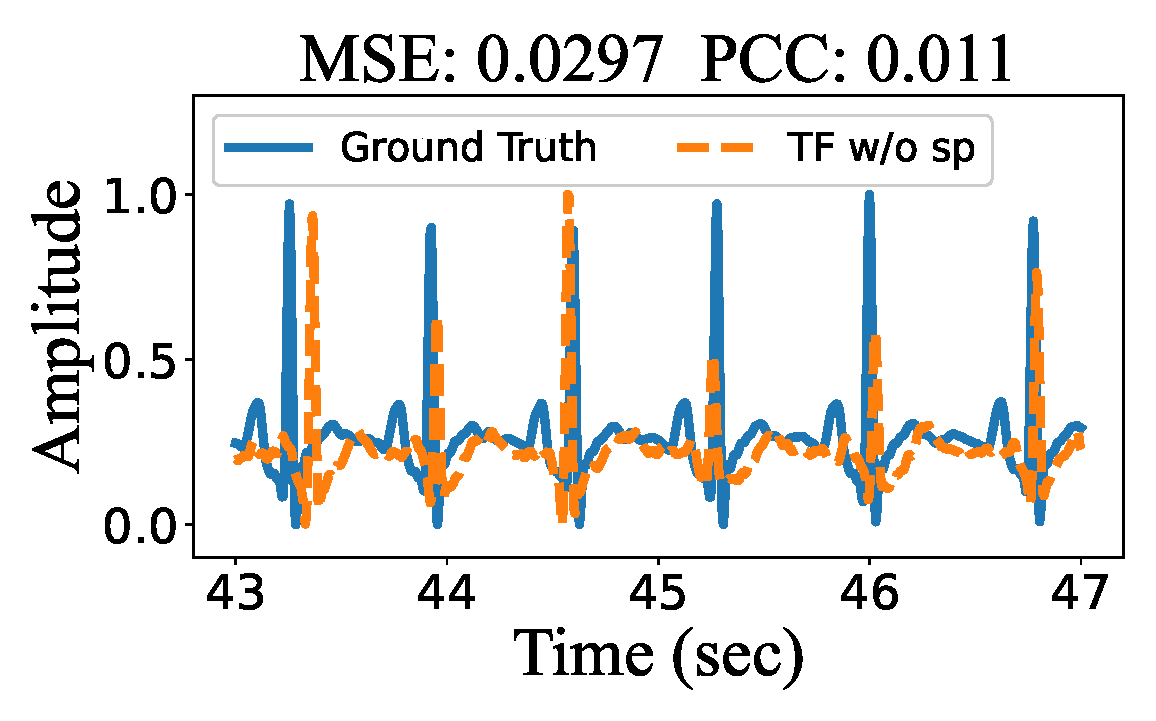
\includegraphics[width=0.3\columnwidth]{fs_bad.eps}}
  \subfloat[]{\label{fig:fs_good}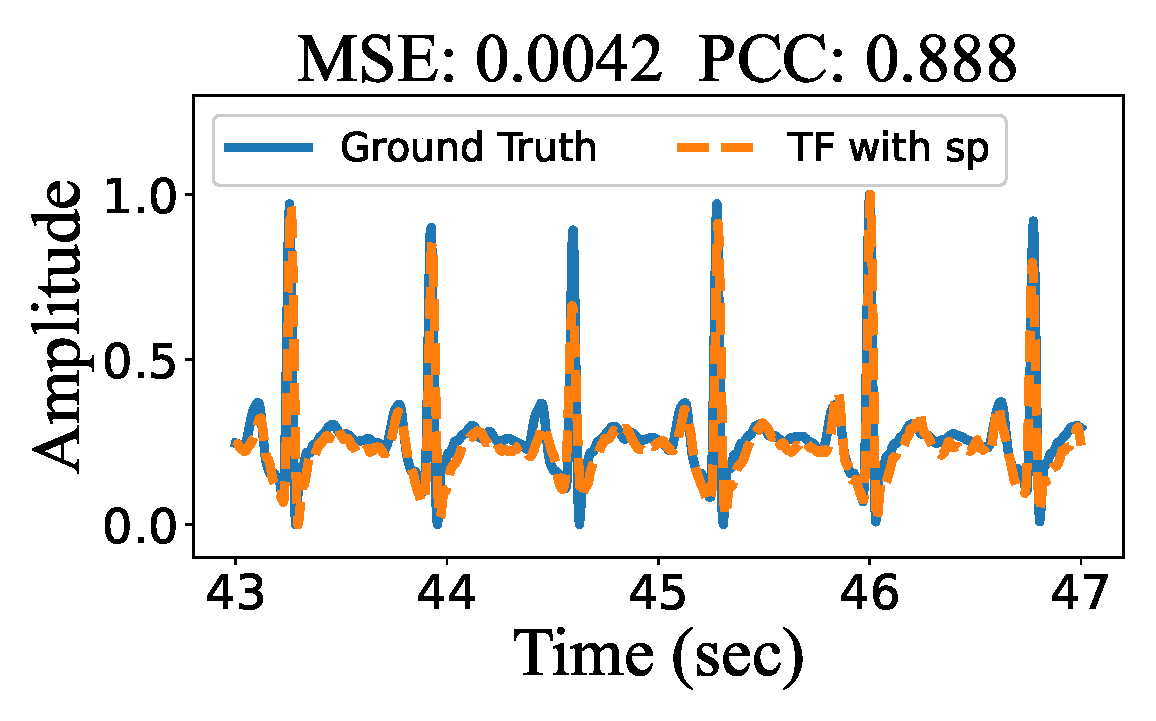
\includegraphics[width=0.3\columnwidth]{fs_good.eps}}
  \caption{Results of transfer learning using limited labeled data: (a) Poor ECG recovery without proper morphological feature and peak location; (b) Good ECG recovery owing to the pre-trained model.}
  \label{fig:fs_res}
\end{figure}

\subsubsection{Summary of Transfer-learning-based ECG Recovery}
Previous evaluations in terms of SSL and fine-tuning stages have illustrated the ability of the proposed RFcardi to learn from unlabeled data and transfer the knowledge to the ECG recovery task using limited radar-ECG pairs. The overall performance in Table~\ref{tab:ecg_few_shot} are plotted in Figure~\ref{fig:overall} for a straightforward comparison:
\begin{itemize}
  \item The performance of supervised learning drops heavily and cannot ensure high-quality ECG recovery after reducing $40\%$ labeled dataset.
  \item Transfer learning could enhance the performance of ECG recovery for the cases with ample labeled training data, and the quality of the pre-trained model has a minor effect on the final result because the deep learning model could learn from numerous radar-ECG pairs.
  \item For the cases with limited labeled data ($40\%$, $60\%$), the proposed RFcardi shows outstanding performance owing to the representations learned from unlabeled data. Furthermore, the quality of the pre-trained model does matter to alleviate the burden of deep learning model to learn both morphological ECG patterns and peak locations, as indicated by the increasing gap between orange and green lines in Figure~\ref{fig:overall}.
\end{itemize}

\begin{figure}[tb]
  \centering
  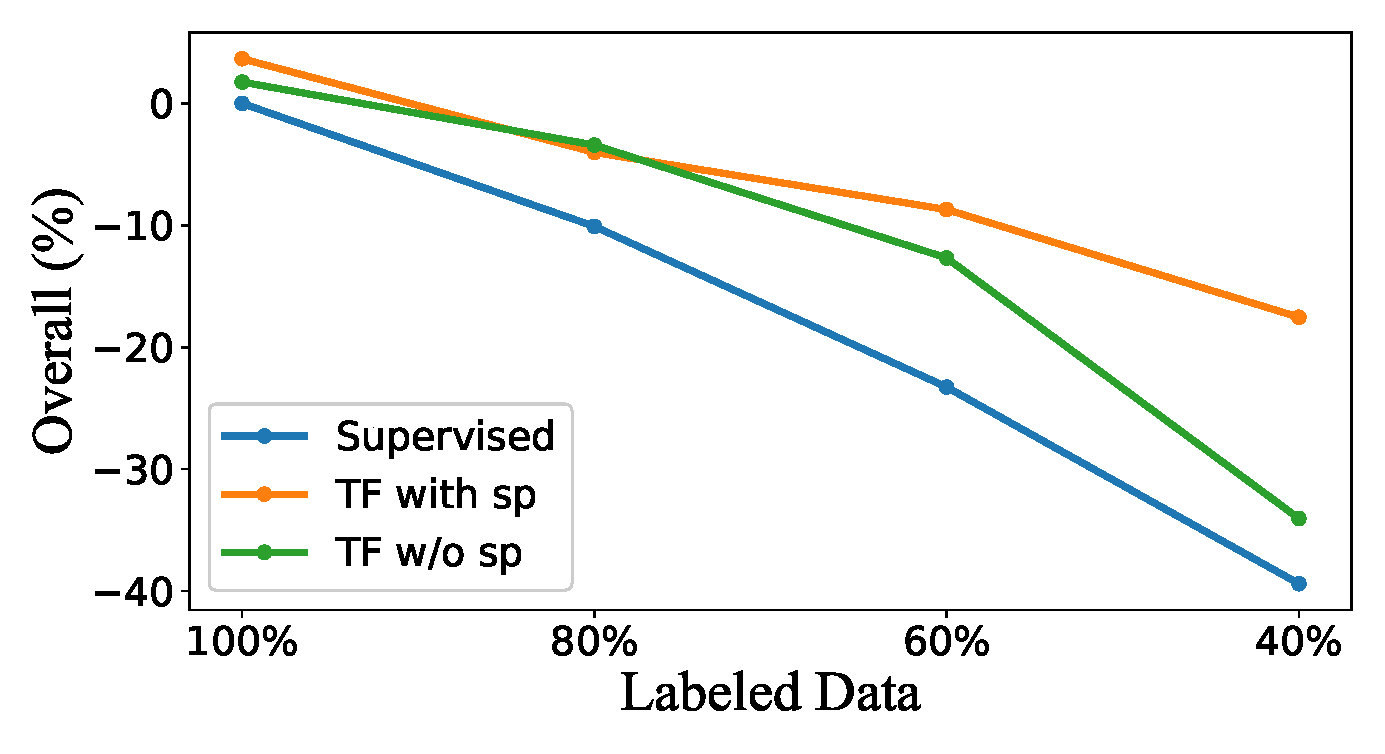
\includegraphics[width=0.6\columnwidth]{overall.eps}
  \caption{Overall performance of the radar-based ECG recovery.}
  \label{fig:overall}
\end{figure}

\section{Conclusions}\label{sec:conclusions}
This paper investigates the efficient collection of high-SNR radar signals with ample cardiac features for transfer-learning-based ECG recovery. Previous methods adopted signal accumulation or clustering to suppress the noises, while the rough localization based on FMCW radar cannot accurately reveal the chest region, requiring a time-consuming traverse among a 3D space for compensation. In this paper, a novel CFT algorithm is proposed to dynamically articulate the points with the best SNR and could track the cardiac location over time if the subjects change posture. In addition, a transfer learning framework RFcardi is designed with SSR as a pre-text task for pre-training to reduce the dependency on cumbersome ECG ground truth collection. The experiments performed in different scenarios prove the feasibility of the CFT-RFcardi framework in radar signal extraction and ECG recovery with limited labeled data, enabling a convenient deployment in new scenarios with limited data for future contactless wellness monitoring.